% ===========================================================================
% A Minor Greenhouse-Gas Sector and the Dominant Particulate Source:
% Residential Fuel Combustion in Pakistan
%
% Target journal: Environmental Modelling & Software (Elsevier)
% Document class: elsarticle, 5p layout
% ===========================================================================

\documentclass[5p,times,authoryear]{elsarticle}

% ===========================================================================
% Shared preamble for every manuscript in this repository.
%
% Papers using it:
%   paper/            agriculture inventory
%   paper_nowcast/    agricultural nowcasting
%   paper_national/   the nine-sector national inventory
%   notes/<sector>/   one data note per non-agriculture sector
%
% It exists because paper/ and paper_nowcast/ began as copies of one another
% and had already drifted five lines apart before a third manuscript existed.
% Eleven copies would drift eleven ways, and a macro that renders differently
% in two papers is the kind of defect nobody notices until proof stage.
%
% \graphicspath is deliberately NOT set here - each manuscript sets its own
% after \input{...preamble}, because figures live beside the document.
% ===========================================================================

\usepackage[utf8]{inputenc}
\usepackage[T1]{fontenc}
\usepackage{amsmath,amssymb}
\usepackage{graphicx}
\usepackage{booktabs}
\usepackage{multirow}
\usepackage{siunitx}
\usepackage[colorlinks=true,citecolor=blue,linkcolor=blue,urlcolor=blue]{hyperref}
% Document-information metadata for every PDF in the bundle (the seventh review noted
% the shipped PDFs carried none). Documents that set their own \hypersetup{pdftitle=...}
% keep it - hyperref takes the LAST setting, and this shared block runs first. Full
% tagged-PDF (tagpdf / \DocumentMetadata) is deliberately not attempted here: the
% installed LaTeX toolchain's support is not uniform across sixteen documents, and a
% half-tagged bundle is worse than an honestly untagged one; deferred deliberately.
\hypersetup{
  pdfauthor={Rehan Ahmad, Pakistan Air Quality Initiative (PAQI)},
  pdfsubject={A reproducible ten-sector national greenhouse-gas inventory
              for Pakistan},
  pdfkeywords={Pakistan, greenhouse gas inventory, IPCC 2006 Guidelines, MRV,
               reproducible research, emissions, air pollutants},
}
\usepackage{caption}
\captionsetup[table]{position=below}
\usepackage{enumitem}
\usepackage{xcolor}
\usepackage{float}
\usepackage{placeins}
\usepackage{tabularx}
\usepackage{natbib}
\usepackage{tikz}
\usetikzlibrary{arrows.meta,positioning,fit,backgrounds}

\setlength{\emergencystretch}{3em}

% Looser float placement to prevent pile-up in two-column mode.
\renewcommand{\topfraction}{0.95}
\renewcommand{\bottomfraction}{0.85}
\renewcommand{\textfraction}{0.05}
\renewcommand{\floatpagefraction}{0.85}
\setcounter{topnumber}{4}
\setcounter{bottomnumber}{3}
\setcounter{totalnumber}{6}

% ---------------------------------------------------------------------------
% Custom shorthand: in macros.tex since the ESSD re-targeting, because the national
% article compiles under the Copernicus class and cannot take this preamble (the class
% loads its own packages) but needs exactly the same macros. This file inputs it so that
% every other manuscript keeps compiling unchanged.
%
% THREE relative paths, because \input resolves against the COMPILE DIRECTORY and not
% against this file, so the depth is a property of whoever is building:
%   ../paper_common      a manuscript compiled from one level down
%   ../../paper_common   papers/<sector>/ and notes/<sector>/
%   ../../../paper_common  paper_national/versions/<v>/, since the national paper was
%                          versioned - that move is what added this third arm, and the
%                          supplement failed with "../../paper_common/macros.tex not
%                          found" until it was here
% A fourth depth needs a fourth arm, which is the cost of keeping a bare `latexmk` in a
% manuscript directory working without a TEXINPUTS set for it.
% ---------------------------------------------------------------------------
\IfFileExists{../paper_common/macros.tex}%
  {\input{../paper_common/macros}}%
  {\IfFileExists{../../paper_common/macros.tex}%
    {% ===========================================================================
% paper_common/macros.tex - the shorthand every manuscript shares.
%
% Split from preamble.tex in the ESSD re-targeting: the national article now compiles
% under the Copernicus class, which loads its own packages and forbids most of what
% preamble.tex sets (geometry-like options, a second hyperref, placeins), but it needs
% exactly the same shorthand as the sector reports. The macros therefore live here, on
% their own, and preamble.tex inputs this file so that every other manuscript keeps
% compiling unchanged. A macro that renders differently in two documents is the defect
% this file exists to prevent; define it once.
%
% Requires: siunitx (for \DeclareSIUnit and \si) - the caller loads it.
% ===========================================================================

% Gas and pollutant names.
\newcommand{\COtwo}{CO\textsubscript{2}}
\newcommand{\COe}{CO\textsubscript{2}e}
\newcommand{\CHfour}{CH\textsubscript{4}}
\newcommand{\NtwoO}{N\textsubscript{2}O}
\newcommand{\NHthree}{NH\textsubscript{3}}
\newcommand{\NOx}{NO\textsubscript{x}}
\newcommand{\SOtwo}{SO\textsubscript{2}}
\newcommand{\PM}{PM\textsubscript{2.5}}
\newcommand{\MCF}{MCF}
\newcommand{\Mt}{\text{Mt~\COe}}
\newcommand{\tCha}{\si{\tonne\per\hectare}}
\newcommand{\AFOLU}{AFOLU}
\newcommand{\GLW}{GLW\,4}
\newcommand{\EFone}{EF\textsubscript{1}}

% siunitx: allow Mt, Tg, ha, head, yr, dB
\DeclareSIUnit{\head}{head}
\DeclareSIUnit{\yr}{yr}
\DeclareSIUnit{\dB}{dB}

% A file name is the one long unbreakable token these documents are full of -
% \texttt{waste\_air\_pollutants\_2024.csv} is wider than a two-column measure and TeX prints
% it past the margin rather than breaking it. Allowing a break AFTER each escaped underscore
% costs nothing and inserts no hyphen, which matters: a hyphenated file name is a wrong file
% name. This is one line because every such name in every document is written with \_.
\let\pkinvunderscore\_
\renewcommand{\_}{\pkinvunderscore\allowbreak}
}%
    {\input{../../../paper_common/macros}}}
% Long unbreakable strings - output filenames, module paths, URLs in \texttt - do not fit a
% two-column measure and TeX prints them past the margin rather than breaking them. Nothing
% read the log, so 47 of those overruns shipped across seven documents. Emergency stretch lets
% the paragraph loosen instead, and \texttt is taught to break at the punctuation these names
% actually contain.
\emergencystretch=6em


\graphicspath{{figures/}}

% ---------------------------------------------------------------------------
\journal{Environmental Modelling \& Software}
% ---------------------------------------------------------------------------

\begin{document}

\begin{frontmatter}

\title{PakEmis Sector Technical Note TN05\\[4pt]
A Hybrid Survey- and Supply-Constrained Residential Greenhouse-Gas and
Air-Pollutant Inventory for Pakistan with Cross-Sector Biomass Accounting}

\author[paqi]{Rehan Ahmad\corref{cor1}}
\ead{rehan@pakairquality.com}

\address[paqi]{Pakistan Air Quality Initiative (PAQI), Karachi, Pakistan}

\cortext[cor1]{Corresponding author}

% --- Abstract ---
\begin{abstract}
This technical note documents household fuel and co-emissions in the shared PakEmis national inventory, whose common annual core spans July 2015--June 2025. Official fuel deliveries, household surveys and agricultural material flows support separate reference S and alternative L configurations. Reference S uses survey-reconstructed household dung; L assumes all agricultural-ledger diverted dung is burned in households. Conservation establishes diverted material but does not determine its destination, so the unresolved quantity remains explicit.

The reference household module contributes \SI{\SectorRefGHG}{\mega\tonne} \COe{} on AR5 GWP-100 and \SI{\SectorRefPMfine}{\kilo\tonne} primary PM$_{2.5}$ in FY2023--24. FY2024--25 quantities are \SI{\SectorLatestGHG}{\mega\tonne} and \SI{\SectorLatestPMfine}{\kilo\tonne}, respectively. Pollutants are native masses; BC and OC are particulate components. Biomass factors use dry fuel including ash and fossil factors retain their applicable energy and particulate definitions.

Historical survey interpolation, stove/fuel factor transfer and structural dung fate remain important limitations. Conditional uncertainty shares activity across gases and pollutants, with ledger dung following the same sampled herd as manure accounting. Spatial products allocate the supported quantities on documented household proxies. Emissions are reported at the appliance; outdoor escape and exposure are not estimated. The note supplies a consistent source account for GHG and air applications without converting emission rankings into exposure priorities.

\end{abstract}

\begin{keyword}
residential fuel combustion \sep household biomass \sep dung cake \sep black carbon \sep
particulate matter \sep cross-sector closure \sep biomass memo convention \sep
IPCC 2006 Guidelines \sep Pakistan \sep household air pollution
\end{keyword}

\end{frontmatter}

%% Generated by scripts/make_release_cover.py; says which release this documents.
% The Sector Technical Note banner (v1.0.0). Each sector manuscript is a PakEmis Sector
% Technical Note, numbered TN01-TN10 in src/pkinv/release.py (TECHNICAL_NOTES), and says
% so on its first page: it documents ONE sector module of the release named in the block
% that follows, and the national totals are stated only in the data-description article
% (the cover block below reproduces them as release identity, not as a claim of this note).
% Usage, in the document body before the release cover:  \TNBanner{TN01}
\providecommand{\TNBanner}[1]{%
  \noindent\fbox{\parbox{\dimexpr\linewidth-2\fboxsep-2\fboxrule}{%
    \textbf{PakEmis Sector Technical Note #1.} Technical documentation of one sector
    module of the PakEmis release identified below, deposited with the data as part of the
    documentation record. The national data-description article (\texttt{paper\_national/})
    is the only document that states the national totals as its own result.%
    \InputIfFileExists{../../paper_common/generated_availability_tn}{}{}%
  }}\par\medskip}

\TNBanner{TN05}
%% GENERATED by scripts/make_release_cover.py from outputs/release_manifest.json.
%% Do not edit: the edit will be overwritten and CI diffs the result.
\newcommand{\ReleaseCover}{%
\begin{center}\small
\setlength{\fboxsep}{4pt}%
\fbox{\begin{minipage}{\dimexpr\linewidth-2\fboxsep-2\fboxrule\relax}\footnotesize
\textbf{Release provenance.} This document describes PakEmis under the period, configuration and source boundaries specified in its methods. The identifiers below link it to the accompanying products and source register.\\[2pt]
\begin{tabular}{@{}p{0.32\linewidth}@{\hspace{0.03\linewidth}}p{0.65\linewidth}@{}}
Release version & \texttt{1.0.0rc69} \\
Commit & \texttt{d8d874622f9a} \\
Reporting period & July 2015--June 2025 (ten fiscal years) (2015-07-01 to 2025-06-30) \\
Reference & S\_TAN (household survey; TAN nitrogen) \\
FY2023--24 total & 444.61 Mt \COe{} (AR5) under S\_TAN, the reference; 449.85 Mt under L\_TAN \\
Release manifest & \texttt{ac0ffe93ad9fcd88} (SHA-256 of \texttt{outputs/release\_manifest.json}, first 16) \\
Source manifest & \texttt{c1be6d314cfce1ea} (SHA-256 of \texttt{data/manifests/source\_manifest.csv}, first 16) \\
Data-description article & \texttt{paper\_national/} (ESSD, in preparation), same release
\end{tabular}
\end{minipage}}
\end{center}}

\ReleaseCover

% ---------------------------------------------------------------------------
% Main body
% ---------------------------------------------------------------------------

% ===========================================================================
\section{Introduction}
\label{sec:introduction}
% ===========================================================================

Household fuel is the sector where greenhouse-gas accounting and air-quality accounting most
clearly disagree about what matters.

Under the IPCC conventions, burning dung and firewood is a modest source: the \COtwo{} is
biogenic and reported outside the national total, leaving only the methane and nitrous oxide
of incomplete combustion. Under a primary-emission lens the same combustion is among the dominant sources of
primary particulate in the country, emitted at breathing height inside and around
dwellings by the population least able to avoid it---though translating emitted mass
into exposure requires evidence this inventory does not carry
(Section~\ref{sec:limitations}).

Both accounts are correct. They are answering different questions, and a sector that is
\SI{5.4}{} or \SI{6.5}{\percent} of Pakistan's emissions (under the survey-based reference and
the all-diverted dung configuration of Section~\ref{sec:results}) and, under either, one of
the largest sources of its primary particulate is where the difference between those
questions has the largest practical consequence.

\subsection{What this paper does}

We report Pakistan's residential fuel combustion for FY2023--24 from national fuel supply
statistics and household-survey quantities, with an air-pollutant layer computed from the same fuel quantities, and treat the
comparison between the two as the result rather than as an aside. Throughout,
``layers'' distinguishes the greenhouse-gas from the air-pollutant calculation,
``configurations'' the two dung activity bases (S, the reference, and L), and ``scenarios'' the
structural sensitivity cases; the word inventory refers to the whole system.

The comparison is defensible here in a way it usually is not. Cross-source particulate
comparisons in developing countries are typically assembled from separate studies with
separate activity bases, so the ratio between two sources is partly an artefact of which
datasets each author had. Every air layer in the inventory this sector belongs to is computed
from that sector's own greenhouse-gas activity data---the same fuel, the same tonnage, the
same population panel---so the ratio between household fuel and road transport
reported in Section~\ref{sec:air} (\numrange{49}{109} across the two dung
configurations) is free of the mismatched-activity artefact, though it remains
conditional on the stated factor, boundary and configuration choices.

\subsection{A transfer that had nowhere to go}

The sector also makes explicit a gap that had been open in this inventory and is common in others.
Pakistani households burn cattle and buffalo dung, and the agriculture sector accounts for
that on the supply side: it removes \SI{28}{\percent} of cattle and \SI{30}{\percent} of
buffalo excreted nitrogen from the manure-management balance and reports it with the notation
key IE---included elsewhere.

Until a residential sector existed, nowhere was elsewhere: \SI{1.259}{\mega\tonne} of
excreted nitrogen a year left one balance correctly and entered no other. The ledger now
conserves that diverted quantity---what agriculture removes is accounted for exactly once,
as household combustion or as a typed unresolved remainder---while the \emph{destination}
of the diverted mass is treated as an
open question: the reference books to household combustion the consumption the household
survey observes, leaving \SI{47.8}{\mega\tonne} with no observed destination, outside the
total; configuration L, the reference of earlier releases, books it all to household
combustion
(Section~\ref{sec:methods}).

\subsection{Contributions}

\begin{enumerate}[leftmargin=*,itemsep=2pt,topsep=3pt]
\item \textbf{A fuel-anchored household energy inventory for Pakistan} across nine streams,
  with no household-count model and therefore nothing that can drift from the fuel actually
  supplied (Section~\ref{sec:methods}).
\item \textbf{An executable cross-sector dung ledger} that conserves the quantity
  diverted from manure management while distinguishing the observed household
  destination from an unresolved remainder (\ref{app:dung}).
\item \textbf{Greenhouse gases and air pollutants on one activity basis}, which is what makes
  the source ranking in Section~\ref{sec:air} a physical statement rather than a
  data-availability artefact.
\item \textbf{An explicit treatment of the biomass memo convention}, under which
  \SI{65}{\percent} of household energy produces \SI{24}{\percent} of reported emissions, and
  of the \SI{65}{\mega\tonne}-scale biogenic \COtwo{} that sits outside the total.
\item \textbf{A survey-anchored firewood quantity}---the HIES 2024--25 design-weighted
  household measurement, corroborated by the independent 2018--19 round and by FAOSTAT's
  moisture-matched equivalent, replacing the flagged FAO estimate the sector previously
  rode---with the sensitivity still published rather than a single number
  (Section~\ref{sec:results}).
\end{enumerate}

Method shared with the other nine sectors is documented separately
\citep{ahmad2026national}.

% ===========================================================================
\section{Related Work}
\label{sec:related}
% ===========================================================================

\subsection{Household energy inventories and their activity problem}

Residential fuel inventories are usually built one of two ways: from a household survey giving
fuel use per household by fuel and region, or from national fuel supply attributed to the
domestic sector. Surveys give richer structure and are expensive and infrequent; supply
statistics are annual and coarse.

Pakistan has both in principle. The Pakistan Social and Living Standards Measurement survey
carries household fuel questions, and OGRA publishes gas and petroleum supply by consuming
sector. This inventory uses the supply route for the fuels that pass through a market, for the
same reason the transport sector does:
the quantity that a national inventory must reproduce is the fuel the country consumed, and a
survey-based estimate has to be reconciled against it afterwards.

The weakness of that choice is specific and is treated in Section~\ref{sec:limitations}: supply
statistics cover fuels that pass through a market, and the two largest household biomass fuels in
Pakistan---firewood and dung---largely do not; for those two the household survey is the estimate.

\subsection{Household air pollution in South Asia}

Solid-fuel combustion in households is among the most studied exposure pathways in the region,
and the health literature on it is far stronger than the emissions literature. What is
comparatively weak is the link between the two: exposure studies measure concentrations in
and around dwellings, while emission inventories estimate mass released, and translating
between them requires assumptions about ventilation, stove type and time-activity patterns
that neither literature settles.

This paper does not attempt that translation. It reports emitted mass on the same activity
basis as the greenhouse gases, which is what an inventory can defensibly supply, and treats
the exposure implication as a ranking of sources rather than a concentration estimate.

\subsection{Emission factors for biomass cookstoves}

The Andreae compilation \citep{andreae2019} and the Akagi compilation \citep{akagi2011}
are the standard field-measurement syntheses for biomass combustion, and the EMEP/EEA
small-combustion chapter \citep{emep2023smallcombustion} is the standard source for
residential fossil fuels. All carry wide ranges, because cookstove emissions depend heavily
on stove design, fuel moisture and operator behaviour, and because measurement campaigns
disagree.

The World Bank's 2024 Pakistan Energy Survey \citep{worldbank2024mtf}, built on a
nationwide 2021--22 Multi-Tier Framework survey, publishes the national stove typology
this literature previously lacked: main-stove shares by locality and province, a
clean-fuel main-stove share of \SI{44.3}{\percent}, rural dominance of traditional and
three-stone/open-fire stoves (\SI{71.8}{\percent}), and stove stacking at
\SI{6.2}{\percent}. It stops short of the fuel-by-device-by-end-use crosswalk a fully
technology-resolved emission inventory needs, which is how this paper uses it: as the
evidence base for a declared technology-mix sensitivity rather than a resolved device
layer.

The biomass particulate and black carbon factors used here come from Andreae's compilation,
the fossil factors from the EMEP/EEA chapter, and the crop-residue rows mirror the
field-burning factors \citep{emep2019} the agriculture sector already uses---one
compilation family per burning layer, but literature values rather than Pakistani
measurement throughout, which is the layer's principal limitation and is stated as such.

\subsection{The biomass \texorpdfstring{\COtwo{}}{CO2} convention}

IPCC reports \COtwo{} from biomass combustion as a memo item outside national totals, on the
reasoning that the carbon was removed from the atmosphere by the plant and its release is part
of a short cycle, with any net loss of biomass stock accounted in the land sector instead.
Methane and nitrous oxide from the same combustion are counted in full, because they are
different molecules with different radiative effects and no corresponding uptake.

The convention is standard and Pakistan's own national submission states it for the same fuels
\citep{pakbur1}. It is worth spelling out here because it produces a result that reads oddly
without it: biomass is \SI{65.4}{\percent} of household energy in this sector and
\SI{24}{\percent} of its reported emissions.

% ===========================================================================
\section{Study Area and Data}
\label{sec:data}
% ===========================================================================

\subsection{Nine streams, four provenances}

The nine fuel streams divide into four provenance classes, and the class determines how
much of this paper each stream needs. The metered fossil streams (natural gas, LPG,
kerosene) are read from regulator and industry sales tables and are essentially settled;
the survey-anchored streams (firewood, dung cake, coal, charcoal) take their quantities from
design-weighted HIES microdata; the ledger-derived stream (crop residues, and dung cake
under configuration L) is computed from the agriculture sector's mass balances rather than observed; and the
expenditure-derived generator stream is priced out of the survey's fuel spending. Table
\ref{tab:fuel} gives each stream's energy contribution and source; the rest of this
section treats the streams in declining order of the scrutiny their provenance demands.

\begin{table}[htbp]
\centering
\footnotesize
\begin{tabular}{@{}lrrl@{}}
\toprule
\textbf{Stream} & \textbf{TJ} & \textbf{\%} & \textbf{Source} \\
\midrule
Dung cake     & 126\,827 & 13.6 & HIES rounds, interpolated \\
Firewood      & 360\,873 & 38.7 & HIES 2024--25 quantities \\
Natural gas   & 284\,553 & 30.5 & OGRA domestic sales \\
Crop residues & 122\,192 & 13.1 & Agriculture residue ledger \\
LPG           &  33\,948 &  3.6 & OGRA domestic sales \\
Kerosene      &   1\,079 &  0.1 & OCAC domestic sectoral sales \\
Generators    &   2\,495 &  0.3 & HIES expenditure / petrol price \\
Coal          &     341  & <0.1 & HIES 2024--25 quantities \\
Charcoal      &     246  & <0.1 & HIES 2024--25 quantities \\
\midrule
\textbf{Total} & \textbf{932\,554} & \textbf{100.0} & \\
\bottomrule
\end{tabular}
\caption{Household fuel input, FY2023--24, reference. Four provenances---a cross-sector ledger, a
household survey \citep{hies2025,hies2019}, a metering regulator
\citep{ogra2024,ocacaviation}, and an expenditure-derived stream priced at the
administered petrol rate \citep{goppetrol}---differing in quality by an order of
magnitude; Section~\ref{sec:limitations} treats them separately rather than reporting a
single activity uncertainty.}
\label{tab:fuel}
\end{table}

\begin{figure}[htbp]
\centering
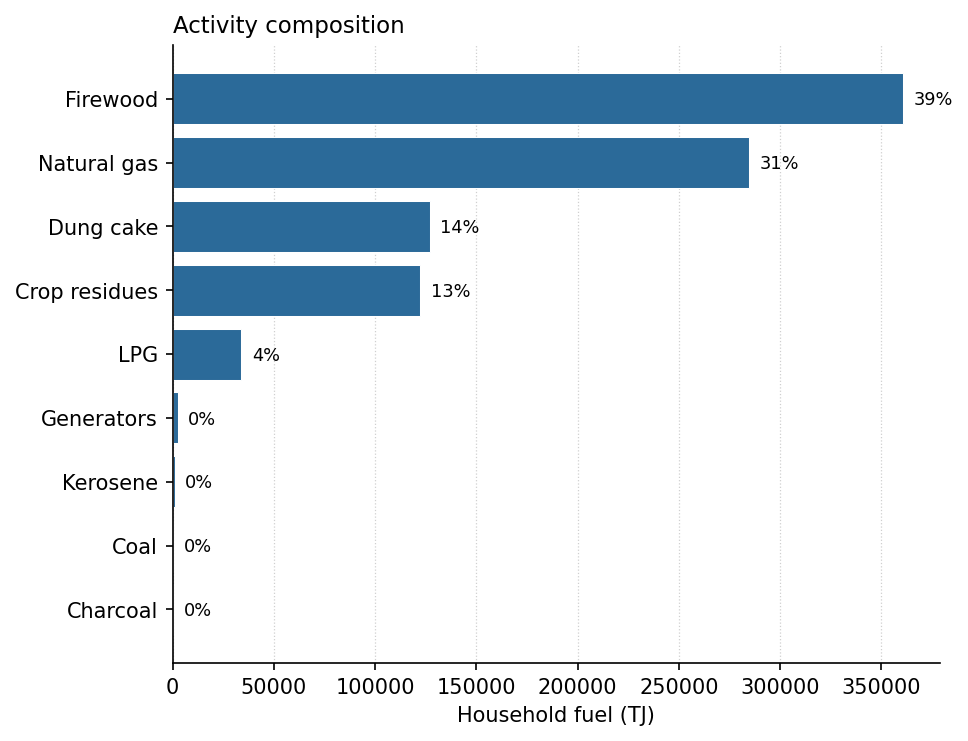
\includegraphics[width=\linewidth]{residential_activity.png}
\caption{Activity composition. Biomass---dung, firewood, crop residues and charcoal together---is \SI{65.4}{\percent} of
household energy, which is the fact behind both the particulate result and the sector's
uncertainty.}
\label{fig:activity}
\end{figure}

\subsection{The fossil streams}

Natural gas, LPG and kerosene are metered, billed and reported by the regulator with a domestic
sector breakdown. They are the best-constrained activity data in the sector and carry
correspondingly narrow uncertainties: \SI{10.8}{\percent} on gas \COtwo{},
\SI{20.9}{\percent} on LPG, \SI{20.2}{\percent} on kerosene.

Natural gas alone is \SI{15.96}{\mega\tonne} of \COtwo{}---\SI{66}{\percent} of the sector's
reported emissions from \SI{31}{\percent} of its energy---because it is the only major stream
whose \COtwo{} is reportable rather than a memo item.

\subsection{Dung cake: one diverted quantity, two destination readings}

The quantity agriculture diverts as dung fuel is derived from that sector's own nitrogen
flow: the same herd, the same species categories, the same burned-fuel shares that drive
agriculture's removal, converted from nitrogen to volatile solids at IPCC's rates for
the same animal categories and region (\ref{app:dung}). The chain runs
\SI{38.77}{\mega\tonne} of ash-free volatile solids $\rightarrow$ \SI{51.69}{} of
total dry solids (ash restored) $\rightarrow$ \SI{58.74}{\mega\tonne} of air-dry cake
(moisture restored, the mass the as-received calorific value pairs with; fractions from
proximate-analysis literature \citep{szymajda2019}; Table~\ref{tab:massbases}).

What that diverted mass does next is read two ways. The reference books to household
combustion the cake households report burning in HIES: the two rounds
(\SI{6.50}{\mega\tonne} in 2018--19, \SI{11.97}{} in 2024--25) anchor a per-household
quantity, interpolated between the rounds and held at the first round's rate before it,
and FY2023--24, which lies between them, takes \SI{10.93}{\mega\tonne}
(\SI{9.62}{} of total dry solids). The remainder's destination is left unresolved,
outside the total. Configuration L books all \SI{58.74}{\mega\tonne} to household
combustion: a destination assumption for the diverted dung, the reference of earlier
releases, and not a reading of household use. Section~\ref{sec:results} carries both.

The survey leaves its own questions open. The two rounds disagree by a factor of
\num{1.53} per household. The design SE of the dung total is \SI{6.6}{\percent} in
2024--25 and \SI{4.1}{} in 2018--19, and in 2024--25 the top 5\% of reporting
households hold \SI{44.7}{\percent} of the reported dung, against \SI{19.6}{} in
the earlier round. The dung activity term therefore carries \SI{35}{\percent}, the
width firewood carries.

\subsection{Firewood, measured by survey}

Firewood is the largest household fuel by energy and the only one with no
supply-side statistic. The quantity used here is the HIES 2024--25 design-weighted
national total \citep{hies2025}---\SI{23.1}{\mega\tonne} of air-dry wood a year entering
households as purchased, own-produced, in-kind or gifted consumption, recorded in kilograms
over a one-month recall for 30,123 households and weighted to the 39.9 million the sampling
frame represents.

One vintage mismatch is explicit rather than smoothed: the survey's field year is July 2024
to June 2025 (each household reporting one month within it), while this inventory's
reference year is FY2023--24. The round is applied to the adjacent fiscal year because it
is the nearest measurement---the alternative is the 2018--19 round, six years out---and
the two rounds' 6~percent agreement bounds what a one-year offset can plausibly move; the
offset is one of the systematic risks the stream's \SI{35}{\percent} uncertainty prices.
The time series (Section~\ref{sec:results}) interpolates per-household quantities between
the rounds rather than pinning either to a year it did not measure.

\begin{table}[htbp]
\centering
\footnotesize
\begin{tabular}{@{}lrr@{}}
\toprule
 & \textbf{2018--19} & \textbf{2024--25} \\
\midrule
Reporting households ($n$)          & 10\,636 & 11\,524 \\
Weighted user households (M)        & 13.0 & 14.0 \\
kg per user household per day       & 4.63 & 4.52 \\
Design SE of the total (\%)         & 2.4$^a$ & 7.1$^b$ \\
Top 1\% of households' share        & 0.05 & 0.19 \\
Top 5\% of households' share        & 0.17 & 0.33 \\
Interview quarters covered          & n/r & 4 of 4 \\
\bottomrule
\end{tabular}
\caption{Firewood survey diagnostics
(\texttt{hies\_diagnostics.csv}). Stratum-clustered linearized SEs: $^a$on the
published PSU; $^b$on an enumeration-block proxy (the 2024--25 release publishes no
PSU variable), so the two are not strictly comparable. The 2024--25 round's heavier
tail---one percent of reporting households carrying \SI{19}{\percent} of the weighted
total, against \SI{5}{} in 2018--19---is the single diagnostic most worth watching;
the per-user-day quantities, in the \SIrange{4.5}{4.6}{\kilo\gram} band both rounds,
are the reassuring one.}
\label{tab:hiesdiag}
\end{table}

Three estimates now bracket the quantity, and their agreement is the basis for trusting any
of them. The independent HIES 2018--19 round \citep{hies2019}, a different sample six years
earlier, gives \SI{22.0}{\mega\tonne}---within \SI{6}{\percent}. FAOSTAT's supply series
\citep{faostat}, the previous anchor for this stream, sits \SI{7}{\percent} above the
survey once its oven-dry basis is moisture-matched. A household self-report and a commodity
supply balance carry different biases, so their convergence is informative in a way
neither alone could be, and the comparison is a published output. FAOSTAT carries FAO's own ``E'' estimate flag in every year since 2009 and does not
move between years, which is why it was demoted to a structural scenario rather than retained
as the estimate.

Section~\ref{sec:results} still reports the sector three
additional ways---excluded, and at $\pm\SI{35}{\percent}$ quantity---so a reader can see
exactly what firewood is worth. The \SI{35}{\percent} carried in the propagation, down from
\SI{60}{\percent} in the FAOSTAT era, is not the survey's sampling error---the
stratum-clustered design SE is \SI{7.1}{\percent} for the 2024--25 round and
\SI{2.4}{} for 2018--19 (Table~\ref{tab:hiesdiag})---but prices what a household survey
cannot see: one-month recall scaled to a year, wood consumed outside the dwelling,
informal-enterprise use booked to households, and the outlier concentration the
diagnostics table quantifies.

\subsection{What is deliberately absent}

Household electricity. At \SI{39728}{\giga\watt\hour} it is the largest single item in every
Pakistani household energy statistic---nearly half of national consumption---and it is not in
this sector, because those emissions are generated at the power station and counted in 1A1a.
Adding them here would double-count roughly a quarter of the national inventory. A test asserts
that no electricity stream exists, so a future edit that "fixes the missing
electricity" is rejected rather than silently inflating the country's emissions.

Household coal and charcoal, once NE here, are now the sector's two smallest streams: the
HIES processing that re-anchored firewood measured them in passing, at \SI{13.2}{\kilo\tonne}
of coal and \SI{8.3}{\kilo\tonne} of charcoal---each reported by about one household in a
thousand, three orders of magnitude below firewood, and roughly a tenth of what the
2018--19 round recorded. With so few reporting households the survey \emph{suggests} a
substantial decline rather than confirms one: the clustered design SEs are
\SI{34}{\percent} on the 2024--25 coal total (23 reporting households, the heaviest
one percent of them carrying \SI{35}{\percent} of it) and \SI{16}{} on charcoal, and
questionnaire harmonisation between rounds has not been audited for these two items.
The decline direction survives intervals that wide; its magnitude does not. The regulator's
nil household coal figure turns out to be roughly right for the wrong reason: not silence,
but a quantity too small for a supply table to resolve. One residue caveat is carried in the conservative direction: the crop-residue stream
is an \emph{upper-bound residential allocation} of the agriculture-ledger fuel destination.
The ledger's fuel fraction covers all fuel use of each residue, not household fuel
specifically---brick kilns and small industry burn cotton sticks too---so
$R_{\text{fuel}} = R_{\text{household}} + R_{\text{commercial/industrial}} +
R_{\text{unresolved}}$, and booking the whole destination to households can only
overstate this sector. The survey's price bracket is the demand-side check that bounds
it, and the HIES expenditure items are the future constraint on the household share. What remains absent is biogas
(digester counts not obtained; NE) and the upstream wood carbonised into the charcoal
(roughly \SI{35}{}--\SI{50}{\kilo\tonne}, booked to the producing category IPCC assigns
it and unestimated nationally).

% ===========================================================================
\section{Methods}
\label{sec:methods}
% ===========================================================================

\subsection{Nine streams, four provenance classes, no household model}

For each stream $s$ and gas $g$,
\begin{equation}
E_{g,s} \;=\; A_s \cdot EF_{g,s},
\end{equation}
where $A_s$ is the national quantity of fuel entering households in terajoules and
$EF_{g,s}$ the IPCC Table~2.5 residential default \citep{ipcc2006stationary}. The nine
streams divide into four provenance classes, and everything else in this section
documents how each class produces its $A_s$: metered-regulatory (natural gas, LPG,
kerosene), survey-primary (firewood, dung cake, charcoal, coal), cross-sector ledger (crop
residues, and dung cake under configuration L), and expenditure-derived (generators).

With one exception there is no household-count model and no per-capita intensity anywhere
in the magnitude
chain: a household model would give structure the supply statistics do not, and would
introduce a quantity that can drift from the fuel actually supplied. The exception is the
reference dung quantity, which is the survey's per-household quantity, interpolated
between the two rounds, times the year's households
(Section~\ref{sec:dungmethod}). Regional and
temporal structure enters only downstream of the national totals---the provincial,
district, grid and monthly layers distribute each stream's fixed national quantity and
reconcile exactly back to it. The transport sector in this inventory makes the same
choice for the same reason \citep{ahmad2026national}.

\subsection{Household-survey processing}
\label{sec:hiesmethod}

Both HIES rounds are processed from the PBS SPSS microdata \citep{hies2019,hies2025}:
the Section~6A consumption module, item codes 045202 (LPG, kg), 045301 (kerosene,
litres), 045401 (firewood, kg), 045402/045403 (charcoal and coal, kg), 045404 (dung
cake, kg), and the value-only items 045102 (generator expenses), 045201 (piped gas),
045405/045406 (agricultural wastes and cotton sticks). Each item carries quantity and
rupee value over four acquisition routes---purchased, wages-in-kind, own-produced, and
gifts or assistance---against a one-month recall; quantities are summed over routes and
annualised $\times 12$ (the 2024--25 round's interviews cover all four quarters, so the
annualisation averages over season). Design weights are the household weight on the
2024--25 person roster and the published PSU weights for 2018--19; weighted household
totals (33.2 and 39.9~million) land on the frame. Own-produced and gifted consumption
carries PBS's imputed rupee value, so item values are consumption values, not purchase
spending. National totals, province~$\times$~urban/rural strata, unit values, and the
diagnostics of Table~\ref{tab:hiesdiag} (design SEs stratum-clustered on the published
PSU or, for 2024--25, an enumeration-block proxy; top-percentile concentration;
per-user-day rates) are all committed as derived tables; the microdata itself is
fetched and hash-pinned, never redistributed.

The outlier policy is diagnosis before exclusion, and kerosene is the worked example:
its 2024--25 item rides 96 reporting households whose implied unit value is a fifth of
the retail price, so the survey figure is published as unusable on the comparison table
and the stream keeps its OCAC sectoral control. No survey observation is trimmed or
winsorised anywhere; concentration is reported (Table~\ref{tab:hiesdiag}) rather than
removed.

\subsection{Mass bases}

Section~\ref{sec:massbases} (Table~\ref{tab:massbases}) states, for every solid fuel,
the reported mass and its basis, the moisture and ash fractions, the energy pairing and
the pollutant-factor mass. The rule: as-received NCVs pair with air-dry mass, per-kg-dry
pollutant factors pair with the dry mass, and no conversion is applied twice.

\subsection{The biomass memo convention, and what it does to the arithmetic}

Biogenic \COtwo{} from dung and firewood is reported outside the national total:
\SI{12682}{\giga\gram} from dung cake, \SI{40418}{\giga\gram} from firewood and
\SI{12260}{\giga\gram} from crop residues and charcoal,
\SI{65359}{\giga\gram} together (\SI{120817}{} under configuration~L). Their \CHfour{} and \NtwoO{}
are counted in full.

The consequence is worth following through, because it produces a result that looks
wrong without the convention. Biomass is \SI{65.4}{\percent} of household energy and
contributes \SI{5.77}{\mega\tonne} of the sector's
\SI{24.22}{\mega\tonne}---\SI{24}{\percent}---entirely as methane and nitrous oxide.
Natural gas is \SI{30.5}{\percent} of the energy and \SI{66}{\percent} of the
emissions, because its \COtwo{} is reportable.

An inventory that reported biomass \COtwo{} inside the total would show this sector at
roughly \SI{90}{\mega\tonne} and would be wrong by IPCC's conventions and by
Pakistan's own stated practice \citep{pakbur1}. An inventory that excluded biomass
\CHfour{} and \NtwoO{} along with its \COtwo{}---a more common error---would show
\SI{18.45}{\mega\tonne} and would miss the incomplete-combustion products that are the
sector's real climate contribution.

\subsection{The dung-cake transfer, and the two configurations}
\label{sec:dungmethod}

The agriculture sector removes \SI{28}{\percent} of cattle and \SI{30}{\percent} of
buffalo excreted nitrogen from its manure-management balance, because that dung is
burned as fuel, and books it IE against Energy. The diverted quantity is that nitrogen
as mass:
\begin{equation}
M_{\mathrm{VS}} \;=\; \sum_{a} N_a \cdot f_a \cdot \frac{\mathrm{VS}_a}{\mathrm{Nex}_a},
\end{equation}
over animal categories $a$, converted to total solids and air-dry cake through the
declared ash and moisture fractions. Configuration~L burns all of it in households. The
reference (configuration~S) instead takes the HIES-reported cake quantity directly---the
per-household quantity interpolated between the two rounds and held at the first round's
rate before it, times each year's households---and removes the same moisture fraction
for its dry mass. The nitrogen equality against
agriculture is asserted with \texttt{==} in either case---it concerns what was
\emph{diverted}, which neither configuration disputes---and the destination identity is
$D_{\text{diverted}} = D_{\text{residential}} + D_{\text{other/unresolved}}$
(Section~\ref{sec:results}; \ref{app:dung}).

\subsection{The crop-residue transfer}

Every crop's above-ground residue mass closes over four destinations in the agriculture
sector's residue ledger,
\begin{equation}
R_{\text{produced}} \;=\; R_{\text{returned}} + R_{\text{field-burned}} +
R_{\text{fuel}} + R_{\text{other}},
\end{equation}
with the fractions summing to one exactly and $R_{\text{other}} \geq 0$ asserted per
crop, so the soils return, the field-burning category and this sector cannot claim the
same tonne twice. The residential stream is $R_{\text{fuel}}$ (\SI{9.27}{\mega\tonne}
dry; half cotton sticks)---an upper-bound residential allocation of the ledger's
fuel destination. Two caveats are declared: the fuel fraction covers all fuel use, not
household fuel specifically ($R_{\text{fuel}} = R_{\text{household}} +
R_{\text{commercial/industrial}} + R_{\text{unresolved}}$; conservative for this
sector), and its values are Tier~2 judgement---so the survey's price bracket, from the residue expenditure items
priced at the survey's own firewood and dung unit values, is published as the
demand-side check (\SIrange{7.8}{24.7}{\mega\tonne} air-dry; the ledger's \SI{10.53}{}
falls inside, asserted by test). The bracket's two ends are priced as named scenarios:
\SI{23.92}{\mega\tonne} for the sector at the low end and \SI{25.78}{} at the high end.

\subsection{The generator stream and its road carve-out}

Generator fuel is the one expenditure-derived stream: the HIES generator-expenses item
(\SI{20.6e9}{} rupees, \SI{0.38}{\percent} of households) over the administered petrol
price \citep{goppetrol}, at standard density, gives \SI{56.3}{\kilo\tonne} of petrol
(\SI{2495}{\tera\joule}), on stationary Table~2.5 factors. Because that petrol is
bought at the same stations the road-transport control counts, it is deducted from the
road petrol control through the same executable closure the railway diesel carve-out
uses (the deduction reads this sector's accessor directly), and a test asserts the
equality---the same litre cannot burn in two
sectors. Declared limits: the expenditure item may sweep in oil and minor maintenance,
the split is assumed all-petrol, and no air-pollutant rows are published (no
household-genset factor class exists).

\subsection{Air-pollutant factors}

Every factor the air layer can burn is a row in the factor file and is rendered,
generated rather than transcribed, in \ref{app:factors}: Andreae field measurements for
the biomass streams \citep{andreae2019}, the EMEP/EEA small-combustion chapter for the
fossil streams \citep{emep2023smallcombustion}, agriculture-mirror rows for residues,
and black carbon as declared fractions of PM$_{2.5}$. The basis rules (mass versus
energy, filterable-condensable caveats, deliberate omissions) are stated there once,
and the source-by-pollutant coverage - every E derived from the layer itself, every
NE with its declared reason - is the air completeness matrix of \ref{app:airmatrix}.
All pollutant masses are gross emission at the appliance (Section~\ref{sec:air}).

\subsection{Uncertainty}

The integrated conditional ensemble samples shared household quantities across native gases and pollutants and retains named source-factor identities. Ledger-L dung follows the same sampled herd as manure accounting; diversion, volatile-solid rates and destination remain conditional assumptions. Structural dung, wood, stove/fuel and survey-construction cases are not sampled into a combined interval and have no assigned probabilities. Paired annual realisations produce trend intervals, with persistent and annually independent activity errors reported separately. Technology endpoints are sensitivities rather than probabilistic residential/road ratio limits. The older sector-local aggregate interval remains a diagnostic and does not replace the current joint parameter product.

\subsection{Spatial hierarchy}

National totals distribute down four levels, reconciling exactly at each:
province~$\times$~urban/rural strata from the HIES quantities; provinces on per-stream
geographies (metered gas connections for piped gas; HIES strata quantities for
firewood, dung, LPG and residues; population for the four thin-sample streams, with
the herd geography retained as dung's structural alternative); districts by the
survey's urban/rural rates on census district populations; and a \SI{0.05}{\degree}
grid on per-stream surfaces (built-up fraction for gas and generators, livestock
density for dung, cropland for residues, population for the rest---declared judgement
of the same class as the railway corridor weights). HIES is representative at
province~$\times$~region, so the within-region district split is population-shaped
until the Census~2023 cooking-fuel tables are processed; the gap register carries them.

\subsection{Time series and monthly profiles}

The FY2015--16 to FY2024--25 series moves gas on a transcribed OGRA
archive \citep{ograarchive} (one interpolated year, labelled), dung and firewood on
per-household quantities interpolated
between the two survey rounds on census-shaped household counts (configuration~L moves
dung on the herd through the fixed nitrogen arithmetic), and residues on crop
production through the fixed ledger; the five minor streams are held at reference
values with basis flags. The reference year is the engine's own output, byte-identical
by construction. Below the year, monthly profiles are synthetic and labelled so:
\begin{equation}
E_{m,f} \;=\; (1 - h_f)\,\frac{E_f}{12} \;+\; h_f\,E_f\,
\frac{\mathrm{HDD}_m}{\sum_{m'} \mathrm{HDD}_{m'}},
\end{equation}
with declared heating fractions $h_f$ per fuel, degree-days from NASA POWER monthly
temperature \citep{nasapower} weighted by each province's share of the sector, and the
generator stream on the cooling-degree shape instead (load-shedding season). Cooking
and other base load is the flat term---the degree-day shape is never applied to it.
Twelve months close to every annual total exactly, asserted on every run; the
base-versus-climate decomposition is a column in the monthly output.

% ===========================================================================
\section{Emission Factors: Table 2.5, Not Table 2.2}
\label{sec:factors}
% ===========================================================================

\subsection{Which of the four tables}

IPCC Volume~2 Chapter~2 publishes four parallel default tables for stationary combustion---
energy industries, manufacturing, commercial, and residential---and this sector must use
Table~2.5, Residential and Agriculture/Forestry/Fishing.

\begin{table}[htbp]
\centering
\footnotesize
\begin{tabular}{@{}lrrr@{}}
\toprule
\textbf{Natural gas} & \textbf{\COtwo{}} & \textbf{\CHfour{}} & \textbf{\NtwoO{}} \\
 & \multicolumn{3}{c}{kg/TJ} \\
\midrule
Table 2.5, residential        & 56\,100 & 5 & 0.1 \\
Table 2.2, energy industries  & 56\,100 & 1 & 0.1 \\
\midrule
\textbf{Kerosene} & & & \\
Table 2.5, residential        & 71\,900 & 10 & 0.6 \\
Table 2.2, energy industries  & 71\,900 &  3 & 0.6 \\
\bottomrule
\end{tabular}
\caption{\COtwo{} is identical because it depends only on the carbon in the fuel. \CHfour{} is
not: residential natural gas is five times the utility value and residential kerosene more than
three times, because a small appliance burns less completely than a power-station boiler.}
\label{tab:tables}
\end{table}

Taking Table~2.2 here would understate household methane by \SI{80}{\percent} while leaving
\COtwo{} exactly correct---and \COtwo{} is \SI{76}{\percent} of the sector's reported
emissions, so every obvious check would still pass. This is one of four instances of the same
trap documented across this inventory \citep{ahmad2026national}; the power sector's module
carries the mirror-image warning, and a test pins the direction in both.

\subsection{Biomass factors, and why their bands are wide}

The dung and firewood streams carry uncertainties above \SI{150}{\percent} on their methane and
nitrous oxide. That is not conservatism: cookstove emission factors genuinely span that range,
because combustion completeness depends on stove design, fuel moisture, feeding rate and
operator behaviour, and measurement campaigns disagree substantially.

The consequence is that the biomass streams that supply most of the sector's energy are also its most
uncertain emission streams, which is why the sector's primary band---the grouped Approach-1
figure of $\pm\SI{23.1}{\percent}$ (Section~\ref{sec:results})---is wide despite three of
the nine streams being metered: the metered gas, LPG and kerosene core is
power-station-grade, and everything around it is not.

\subsection{Fossil and biogenic methane in one category}

This sector is the only one in the inventory that emits both. Dung and firewood methane is
biogenic and takes the AR5 GWP of \num{28}; natural gas, LPG and kerosene methane is fossil and
takes \num{30}. Every methane-emitting component declares which it is, and a contract test
asserts both that the declaration is present and that the \COe{} conversion used the
corresponding value.

The difference is small in this sector---methane totals \SI{5.18}{\mega\tonne} \COe{} of which
\SI{0.05}{} is fossil---but the same field distinguishes landfill methane from combustion
methane elsewhere in the inventory, and a category emitting both is exactly where a missing
flag would be least visible.

\subsection{No separate oxidation factor}

The 2006 Guidelines fold complete oxidation into the emission factor; Table~1.4 carries an
explicit oxidation column of \num{1.0} for every fuel. Applying the 1996-vintage \num{0.98} on
top would double-discount. The waste sector in this inventory \emph{does} carry an oxidation
factor, because open burning genuinely is incomplete, and tests pin both conventions.

% ===========================================================================
\subsection{One mass-basis table for every solid fuel}
\label{sec:massbases}
% ===========================================================================

Three mass bases circulate in this sector---as-received (air-dry), total dry solids, and
ash-free volatile solids---and the superseded dung estimate showed what conflating them
costs. Table~\ref{tab:massbases} states, for every solid fuel, which mass is reported,
which mass the energy calculation burns, and which mass the air-pollutant factors burn,
with the moisture and ash fractions that connect them. The rule it encodes: IPCC's
Table~1.2 net calorific values are as-received and pair with air-dry mass; Andreae-family
pollutant factors are per kilogram of dry fuel including ash and pair with the dry mass;
neither conversion is ever applied twice.

\begin{table*}[tbp]
\centering
\scriptsize
\begin{tabular}{@{}lllllll@{}}
\toprule
\textbf{Fuel} & \textbf{Reported mass} & \textbf{Basis} & \textbf{Moist.\ (ar)} &
\textbf{Ash (dry)} & \textbf{Energy pairing} & \textbf{AP-factor mass} \\
\midrule
Dung cake (S)  & 10.93 Mt & air-dry cake, HIES rounds     & 0.12 & 0.25 &
  air-dry $\times$ 11.6 TJ/Gg (ar) & 9.62 Mt total dry solids \\
Dung cake (L)  & 58.74 Mt & air-dry cake, from N ledger  & 0.12 & 0.25 &
  air-dry $\times$ 11.6 TJ/Gg (ar) & 51.69 Mt total dry solids \\
Firewood       & 23.13 Mt & air-dry wood, HIES 2024--25  & 0.15 & incl.\ in factors &
  air-dry $\times$ 15.6 TJ/Gg (ar) & 19.66 Mt oven-dry \\
Crop residues  & 10.53 Mt & air-dry, from residue ledger & 0.12 & incl.\ in factors &
  air-dry $\times$ 11.6 TJ/Gg (ar) & 9.27 Mt dry matter \\
Charcoal       & 8.3 kt   & as-purchased, HIES 2024--25  & $\sim$0 (declared) & incl.\ in factors &
  as-purchased $\times$ 29.5 TJ/Gg & 8.3 kt taken as dry \\
Coal           & 13.2 kt  & as-received, HIES 2024--25   & --- & --- &
  as-received $\times$ 25.8 TJ/Gg  & energy basis (g/GJ) \\
\bottomrule
\end{tabular}
\caption{Mass bases, fuel by fuel. The reference (S) reads air-dry cake from the survey,
the per-household quantity interpolated between the two rounds, and removes moisture for
its dry mass; under configuration L the dung chain runs
$\mathrm{VS} \rightarrow \mathrm{TS} = \mathrm{VS}/(1-\text{ash}) \rightarrow
\text{air-dry} = \mathrm{TS}/(1-\text{moisture})$ from the nitrogen ledger. The fractions
are the same, so the two configurations differ
only in whose quantity they believe, never in chemistry. Charcoal's as-purchased mass is
taken as dry (lump charcoal equilibrates at a few percent moisture; the conflation is
declared and bounded well below that stream's activity uncertainty). Coal needs no dry
mass because its pollutant factors are on fuel energy. Moisture and ash fractions are
declared literature-range parameters \citep{szymajda2019}, pinned to
\texttt{data/residential\_params.csv} by test.}
\label{tab:massbases}
\end{table*}

% ===========================================================================
\section{Validation}
\label{sec:validation}
% ===========================================================================

\subsection{Against EDGAR, at unmatched scope}

EDGAR reports Pakistani "buildings" at \SI{31.42}{\mega\tonne} \COe{} for 2024
\citep{edgar2025booklet}. This inventory reports \SI{24.22}{\mega\tonne} under the reference
(\SI{77}{\percent} of EDGAR) or \SI{29.47}{} under configuration~L (\SI{94}{\percent}).

The scopes differ in a known direction. EDGAR's buildings category covers residential
\emph{plus} commercial and institutional buildings and stationary agriculture; this sector
covers households only. A households-only estimate should therefore sit below a buildings
estimate, and it does. The remaining \SI{7.20}{\mega\tonne} difference is consistent with
EDGAR's broader non-household scope together with methodological and activity-data
differences; the direction of the comparison is the check, not its magnitude, and the gap
must not be read as a measurement of the commercial sector.

That is a weaker form of validation than a like-for-like ratio, and it is worth being explicit
that the comparison cannot detect an error in either direction of comparable size to the scope
difference. If this sector were \SI{20}{\percent} too low, the ratio would read
\SI{64}{\percent} and would read as a larger scope difference rather than an error.

\subsection{Against Pakistan's own submission}

BUR-1 reports 1A4 for FY2017--18 with a residential component of \SI{19.0}{\mega\tonne},
alongside agriculture at \SI{11.3}{} and commercial at \SI{3.8}{} \citep{pakbur1}. The time
series makes the comparison matched-year: this inventory's FY2017--18 value is
\SI{22.4}{\mega\tonne}, putting the BUR at \num{0.85} of it---consistent with a filing that,
like the CRT below, carries less than the full biomass scope, though the BUR does not publish
its fuel list and the attribution stays a reading, not a finding.

What it does confirm is the convention. Pakistan's own submission states the biomass memo
treatment for the same fuels, so this sector's decision to hold \SI{65347}{\giga\gram} of
biogenic \COtwo{} outside the total follows national practice as well as IPCC's.

\subsection{An executable cross-sector consistency check}

The dung nitrogen equality is asserted, not compared: the quantity this sector's ledger
receives equals the quantity agriculture's manure balance diverts, by construction and
with exact equality, and a test fails if that ever ceases to hold. The equality concerns
what was \emph{diverted}---which both configurations accept---not where it was burned;
under the reference the residual's destination is an open question,
never a conservation failure.

This is a stronger check than any external comparison because it can fail: a change to
agriculture's manure-management shares, its herd, or its volatile-solids rates
propagates here immediately, where two independently computed dung quantities would
drift apart silently and look like two plausible numbers.

\subsection{Against the CRT filing, cell by cell}

Pakistan's first Common Reporting Tables (filed 2024, inventory year 2022) are extracted from
the workbook's own cells on every run, rows found by label, the archive hash pinned by a test.
The headline is a notation key: every Biomass cell in the 1.A.4.b block reads NE. The
country's two largest household biomass fuels---\SI{487700}{\tera\joule} in this inventory,
\num{1.6} times the filing's whole residential activity (more
than three times under configuration~L)---are not estimated in the national
submission at all.

Where the filing and this inventory can meet, they agree. The filing's gaseous row carries
\SI{288493}{\tera\joule} against this inventory's \SI{284553}{} from OGRA's domestic
table---\SI{1.4}{\percent} apart, two derivations of one metered quantity that have never
seen each other. On the filing's own scope and GWPs at the matched straddle-mean year, the
filing reports \SI{17.73}{\mega\tonne} against this inventory's \SI{19.09}{}---within
\SI{8}{\percent}. The biomass NE is therefore a scope statement, not a magnitude dispute:
the two inventories describe the same metered core, and this one adds the fuels the filing
leaves out. Two smaller readings off the same block: the liquid IEFs are a proper
Table~2.5 LPG/kerosene blend (unlike the road-table substitution the railway block of the
same filing carries), and the solid row books \SI{29.5}{\tera\joule} on the lignite factor
set where this inventory carries \SI{341}{} as other-bituminous---both rounding errors on
the sector, recorded rather than smoothed.

\subsection{Against the CCAC assessment, as a closing bridge with a residual}

The CCAC/SEI integrated assessment \citep{ccacsei2023} implies about \SI{224}{\kilo\tonne}
of residential \PM{} for 2021 (\SI{35}{\percent} of a \SI{641}{\kilo\tonne} national
total). The published bridge steps from this inventory's \SI{283}{\kilo\tonne}
(FY2023--24, reference) to that figure through named, quantified wedges: the
inventory year (\SI{24}{\kilo\tonne}, from the time series) and the
residue fuel set (\SI{68}{}), leaving a signed unexplained residual of
\SI{-33}{\kilo\tonne}, \num{-15}~percent of the endpoint: PM definition
(filterable-versus-condensable scope unresolved on both sides), the GAINS factor family
against Andreae field measurements, and remaining activity shares. The bridge closes
exactly by construction; the discipline a test enforces is that the residual exists and
is never redistributed into the named wedges. The bridge has no dung-configuration wedge:
configuration~L at the matched year, \SI{591}{\kilo\tonne}, is a memo row beside it and
not a step of it.

Read as evidence on the configuration choice: after the year wedge alone, configuration~L
stands \num{2.6} times above the assessment, while the reference lands within
\SI{15}{\percent} of it. That is not an adjudication---the CCAC estimate is itself a
model, its household activity is not a measurement, and agreement with one model is weak
evidence---but it is the only independent number that prefers either configuration, and
it prefers S.

\subsection{What is not validated}

The within-province geography: HIES is representative at province and urban/rural level,
so the district layer's within-region split rides census population, and no district fuel
observation tests it. And the air layer's absolute level has no independent Pakistani
emissions measurement---the CCAC comparison above is a model-to-model bridge, ambient
monitoring exists only as concentrations, and translating those to emitted mass requires
dispersion modelling this paper does not attempt.

% ===========================================================================
\section{Results}
\label{sec:results}
% ===========================================================================

\subsection{The sector}

Pakistani households emitted \SI{24.22}{\mega\tonne} \COe{} in FY2023--24 on AR5 metrics
under the reference (\SI{29.47}{} under configuration~L; Table~\ref{tab:configs}), or
\SI{24.06}{\mega\tonne} on AR6, plus \SI{65359}{\giga\gram} of biogenic \COtwo{} reported
as a memo item outside the national total. This subsection's detail tables ride the
reference; every headline is restated under configuration~L in
Table~\ref{tab:configs}.

\begin{table}[htbp]
\centering
\footnotesize
\begin{tabular}{@{}llrrr@{}}
\toprule
\textbf{Stream} & \textbf{Gas} & \textbf{Gg} & \textbf{Mt \COe{}} & \textbf{$\pm$\%} \\
\midrule
Natural gas & \COtwo{}  & 15\,963.42 & 15.963 &  10.8 \\
            & \CHfour{} &      1.42 &  0.043 & 150.3 \\
LPG         & \COtwo{}  &  2\,142.15 &  2.142 &  20.9 \\
Kerosene    & \COtwo{}  &      77.57 &  0.078 &  20.2 \\
Coal        & \COtwo{}  &      32.27 &  0.032 &  40.3 \\
Generators  & \COtwo{}  &     172.93 &  0.173 &  40.2 \\
Dung cake   & \CHfour{} &      38.05 &  1.065 & 154.0 \\
            & \NtwoO{}  &       0.51 &  0.134 & 154.0 \\
Firewood    & \CHfour{} &     108.26 &  3.031 & 154.0 \\
            & \NtwoO{}  &       1.44 &  0.383 & 154.0 \\
Crop resid. & \CHfour{} &      36.70 &  1.027 & 161.6 \\
            & \NtwoO{}  &       0.49 &  0.130 & 161.6 \\
\midrule
\textbf{Total} & & & \textbf{24.222} & \textbf{22.9} \\
\bottomrule
\end{tabular}
\caption{Residential fuel combustion, FY2023--24, AR5. Minor gas rows below
\SI{0.01}{\mega\tonne} are omitted from the table and included in the total. Biomass \COtwo{}
is a memo item and does not appear. The total's $\pm$\SI{22.9}{\percent} combines the rows
as if independent; the sector's primary figure is the grouped Approach-1
$\pm$\SI{23.1}{\percent}, which shares each stream's activity term across its gas rows, and
the national Monte Carlo counterpart is $\pm$\SI{30.4}{\percent}. The last is wider for a
named reason: at parameter level the eight biomass CH\textsubscript{4} and
N\textsubscript{2}O rows' declared widths are superseded by the widths their named factor
and calorific-value parameters imply (\texttt{data/uncertainty\_reconciliation.csv}, the
rc41 dispositions), and mean-preserving lognormal draws skew wider still; all are the same
decomposition under different treatments, not competing estimates.}
\label{tab:results}
\end{table}

\begin{figure}[htbp]
\centering
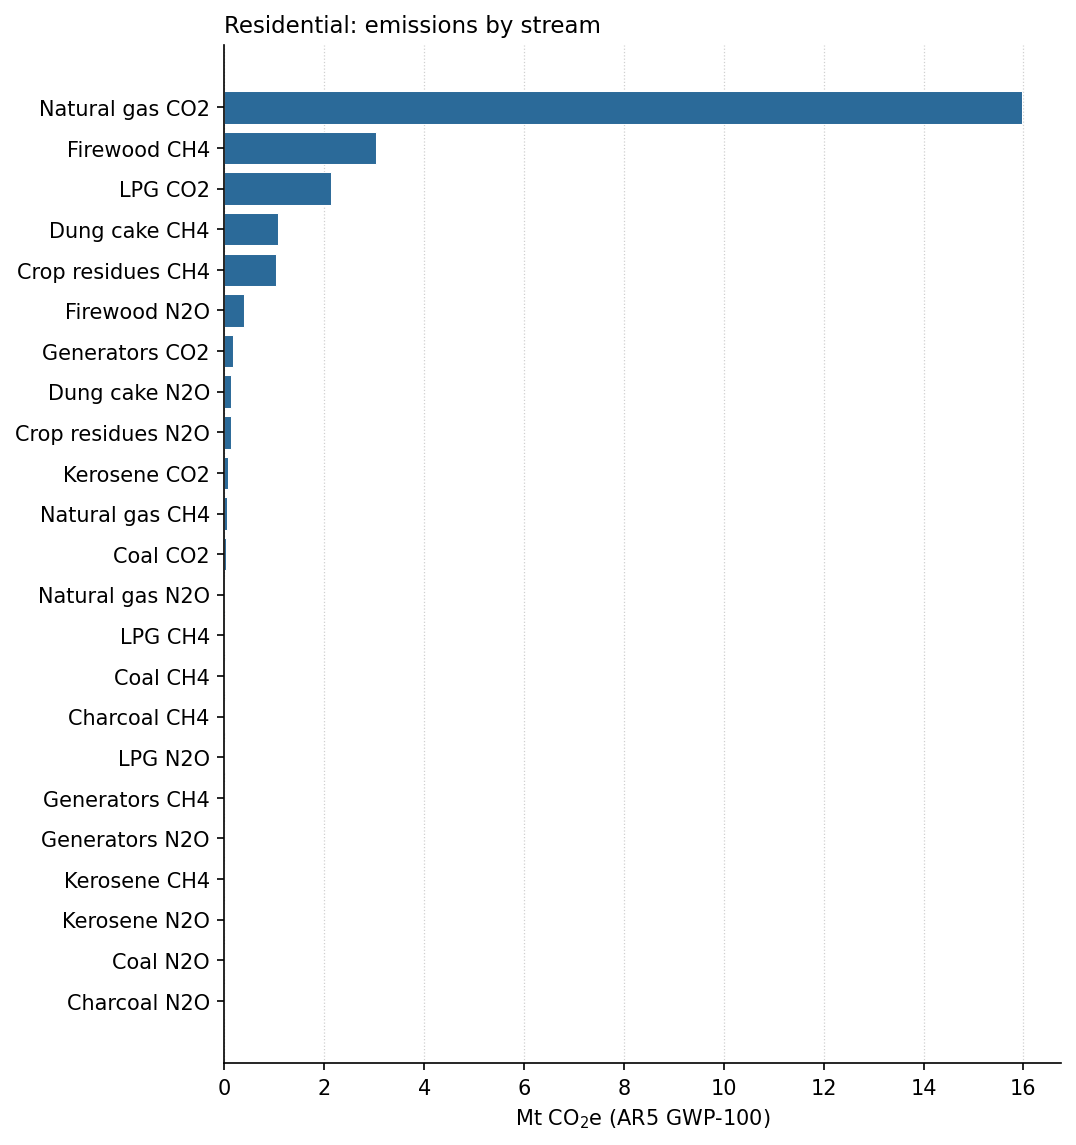
\includegraphics[width=\linewidth]{residential_streams.png}
\caption{Emissions by stream and gas. Biomass streams appear here through their \CHfour{} and
\NtwoO{} only, which is why natural gas carries a far larger share of the emissions than of the
energy.}
\label{fig:streams}
\end{figure}

The inversion between energy and emissions is the central arithmetic result. Biomass supplies
\SI{65.4}{\percent} of household energy and \SI{24}{\percent} of reported emissions; natural
gas supplies \SI{30.5}{\percent} of the energy and \SI{66}{\percent} of the emissions. This is
the biomass memo convention working as intended, and it is why a household-energy statistic and
a household-emissions statistic for Pakistan tell opposite stories about which fuel matters.

\subsection{Firewood, and what it is worth}

\begin{table}[htbp]
\centering
\footnotesize
\begin{tabular}{@{}lr@{}}
\toprule
\textbf{Case} & \textbf{Mt \COe{}} \\
\midrule
Firewood excluded entirely & 20.808 \\
Firewood quantity $-35\%$  & 23.027 \\
Reported                   & 24.222 \\
Firewood quantity $+35\%$  & 25.416 \\
\bottomrule
\end{tabular}
\caption{The sector reported four ways across the firewood cases. Firewood is
survey-anchored since the HIES re-anchoring; the exclusion case bounds what the stream is
worth, and the dung configurations---a larger structural axis---are treated below.}
\label{tab:sensitivity}
\end{table}

\begin{figure}[htbp]
\centering
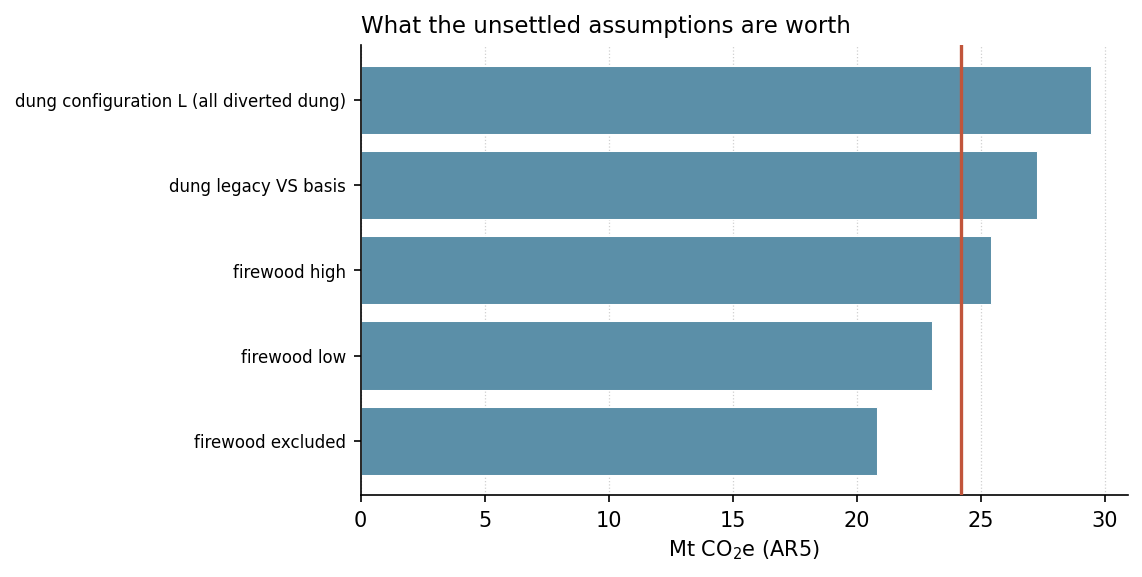
\includegraphics[width=\linewidth]{residential_sensitivity.png}
\caption{The published sensitivity rows as a range around the reported figure. From
lowest to highest: firewood excluded entirely (\SI{20.81}{}), the HIES firewood
quantity $-35\%$ (\SI{23.03}{}) and $+35\%$
(\SI{25.42}{}), the superseded legacy VS dung basis
(\SI{27.28}{}), which is a reading of configuration~L, and configuration~L itself
(\SI{29.47}{\mega\tonne}); the vertical line marks the reference at
\SI{24.22}{\mega\tonne}.}
\label{fig:sensitivity}
\end{figure}

Dropping firewood entirely moves the sector by \SI{14}{\percent}---from \SI{24.22}{} to
\SI{20.81}{\mega\tonne}---which is less than a reader might expect for a fuel supplying
\SI{39}{\percent} of household energy, and the reason is again the memo convention: only
firewood's methane and nitrous oxide are in the total. What exclusion \emph{would} remove is
\SI{40418}{\giga\gram} of biogenic \COtwo{} from the memo and a comparable share of the
air-pollutant layer, where firewood matters most.

\subsection{The survey against the controls}

\begin{table}[htbp]
\centering
\footnotesize
\begin{tabular}{@{}llrrl@{}}
\toprule
\textbf{Fuel} & \textbf{Role} & \textbf{HIES 2024--25} & \textbf{Engine} & \textbf{Ratio} \\
\midrule
Firewood (Mt)   & primary     & 23.13 & 23.13 & 0.94$^b$ \\
Dung cake (Mt)$^c$ & primary  & 10.93 & 58.74 & 0.186 \\
LPG (Mt)        & diagnostic  &  0.90 &  0.72 & 1.248 \\
Kerosene (ML)   & diagnostic  & 77.96 & 30.79 & unusable$^a$ \\
\bottomrule
\end{tabular}
\caption{The published survey-versus-control comparison
(\texttt{residential\_hies\_comparison\_2024.csv}, abridged). Diagnostic ratios are
published and never applied. $^a$The kerosene item rides 116 outlier-heavy households
whose implied unit value is a fifth of retail. $^b$Against FAOSTAT's moisture-matched
equivalent; the survey IS the estimate. $^c$The survey series at the reference year (the
per-household quantity interpolated between the two rounds; the 2024--25 round as
measured is \SI{11.97}{\mega\tonne}) against the dung agriculture diverts, not against
an engine control: the survey IS the estimate, and the ratio is the part of the diverted
supply households are observed burning.}
\label{tab:hies}
\end{table}

The diverted supply is $r_{\text{dung}} = 4.90$ times what households reported in the
2024--25 round, and \num{5.4} times the survey series at the reference year: the nitrogen
ledger implies
\SI{58.7}{\mega\tonne} of air-dry cake, and the survey series puts \SI{10.9}{} in
households. Mass
conservation constrains what agriculture diverted; it is not evidence about the
destination of the conserved mass, and the correct identity is
$D_{\text{diverted}} = D_{\text{residential}} + D_{\text{other/unresolved}}$, not
$D_{\text{diverted}} = D_{\text{residential}}$. The residential row measures what
households burn, and the survey is what observes it; the ledger's burned-fuel shares are
unmeasured Tier~2 values, and nothing held supports a fivefold survey under-count. The
reference is therefore the survey-observed residential-demand configuration
(S), which books the household consumption the survey measures and leaves the
residual's destination unresolved, outside the total. Configuration L, in which the
full diverted quantity is booked to households, was the reference of earlier releases
and is retained beside it as a destination assumption for the diverted dung, not a
reading of household use. The survey is not settled either: it sees only in-scope
household consumption of formed cake, its two rounds disagree by a factor of
\num{1.53} per household, and in 2024--25 the top 5\% of reporting households hold
\SI{44.7}{\percent} of the reported dung (Section~\ref{sec:data}).

\subsection{The reference and configuration L}

\begin{table}[htbp]
\centering
\footnotesize
\begin{tabular}{@{}lrr@{}}
\toprule
 & \textbf{L (all diverted)} & \textbf{S (survey, reference)} \\
\midrule
Dung cake, air-dry (Mt)        & 58.74 & 10.93 \\
Household energy (TJ)          & 1\,487\,257 & 932\,675 \\
Sector \COe{}, AR5 (Mt)        & 29.468 & 24.222 \\
Biogenic memo \COtwo{} (Gg)    & 120\,817 & 65\,359 \\
Primary \PM{} (kt)             & 632.0 & 282.8 \\
Black carbon (kt)              & 41.5  & 20.0 \\
Ratio vs road exhaust \PM{}    & 109.4 & 49.0 \\
National share (\%)            & 6.55  & 5.45 \\
\bottomrule
\end{tabular}
\caption{Every headline quantity under both dung configurations
(\texttt{residential\_configurations\_2024.csv}). S is the reference, and the
detailed spatial and temporal layers are presented under it;
under S, \SI{47.8}{\mega\tonne} of diverted air-dry cake has no observed
destination and is carried as unresolved, outside the total---candidates include
commercial tandoors and eateries, non-household
burning, over-stated burned-fuel shares in the manure-management configuration, field
application, and
survey undercapture of own-produced cake.}
\label{tab:configs}
\end{table}

The configuration choice is the dominant structural axis of the sector: leaving
configuration L for the reference lowers the
total by \SI{5.25}{\mega\tonne}, the particulate headline by more than a factor of two,
and the road-transport ratio from \num{109} to \num{49}. The configurations describe alternative material destinations rather than
a probability interval. Section~\ref{sec:validation} shows the one
external anchor that speaks to it: at the matched year, configuration S sits within
\SI{15}{\percent} of the CCAC/SEI assessment's implied residential particulate, while L
is \num{2.6} times above it.

The \SI{47.8}{\mega\tonne} left unresolved under the reference holds
\SI{1025.6}{\kilo\tonne} of nitrogen and carries no emission. Its candidate
destinations are priced one at a time beside the national total, with no probability
attached (\texttt{national\_dung\_variants.csv}): burned by non-household users,
\SI{5.25}{\mega\tonne} more, which is configuration L reclassified; returned to manure
management, \SI{4.54}{} more; applied to fields, \SI{3.04}{} more.

\subsection{Ten fiscal years and monthly allocation}

The sector reports FY2015--16 through FY2024--25: \SI{21.5}{} to
\SI{22.7}{\mega\tonne}, growth carried by gas connections and the survey-anchored biomass streams, with each
stream's basis recorded with the product. Gas uses nine reported OGRA annual controls
\citep{ograarchive}, including the full FY2024--25 edition, and one labelled
interpolation across the ten-year panel; minor fuel streams remain held. The
matched calendar years this series unlocks are what Section~\ref{sec:validation}'s
official comparisons stand on. For the detailed FY2023--24 reference, a synthetic-labelled monthly layer on
measured degree-days \citep{nasapower} produces a pronounced winter peak that coincides
with Pakistan's smog season---January at \SI{49}{\kilo\tonne} of \PM{} per month
against July's \SI{16}{}---with the generator stream alone running the opposite season
against summer load-shedding. These are allocations of the annual total, not monthly
observations; the output carries the base-load and climate-load components separately,
so the degree-day shape is auditable against the flat cooking term it never touches.

\subsection{Provincial allocation}

\begin{figure}[htbp]
\centering
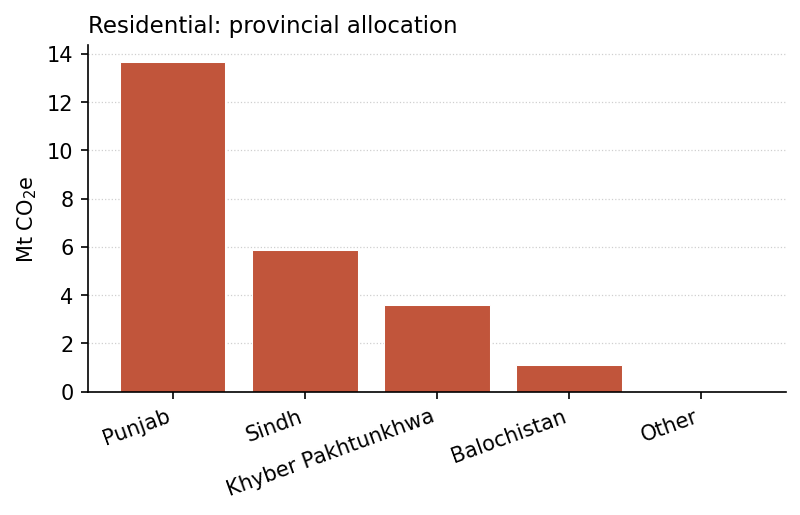
\includegraphics[width=\linewidth]{residential_provincial.png}
\caption{Punjab \SI{13.69}{\mega\tonne}, Sindh \SI{5.86}{\mega\tonne}, Khyber Pakhtunkhwa
\SI{3.58}{\mega\tonne}, Balochistan \SI{1.09}{\mega\tonne}. Each stream rides its own proxy;
the allocation reconciles exactly against each stream's national figure.}
\label{fig:provincial}
\end{figure}

The pattern broadly follows population, as expected for a household sector, with Sindh
somewhat elevated relative to its population share because piped gas connection rates in
Karachi are high and piped gas is the stream whose \COtwo{} is reportable.

\subsection{Districts and the grid}

Below the provinces, each stream's total splits urban/rural by the survey's own rates
and spreads over \num{134} allocation units by the matching population: named
four-province districts and one grouped Other residual for GB/AJK/ICT. These are
allocation units rather than individually observed districts across all territories.
The agricultural account has \num{116} four-province districts plus its grouped Other
unit. The residential summaries reconcile
per province and stream (\texttt{residential\_district\_2024.csv}); Lahore leads at
\SI{2.13}{\mega\tonne} because gas is urban, with Faisalabad (\SI{1.01}{}) and
Rawalpindi (\SI{0.92}{}) behind it. The grid places the same totals at
\SI{0.05}{\degree} on per-stream surfaces, again exactly reconciled
(Figures~\ref{fig:districtmap} and~\ref{fig:gridmap}). These are allocations, not
observations---no district fuel survey exists---and the within-region split stays
population-shaped until the census cooking-fuel tables land
(Section~\ref{sec:methods}).

\begin{figure}[htbp]
\centering
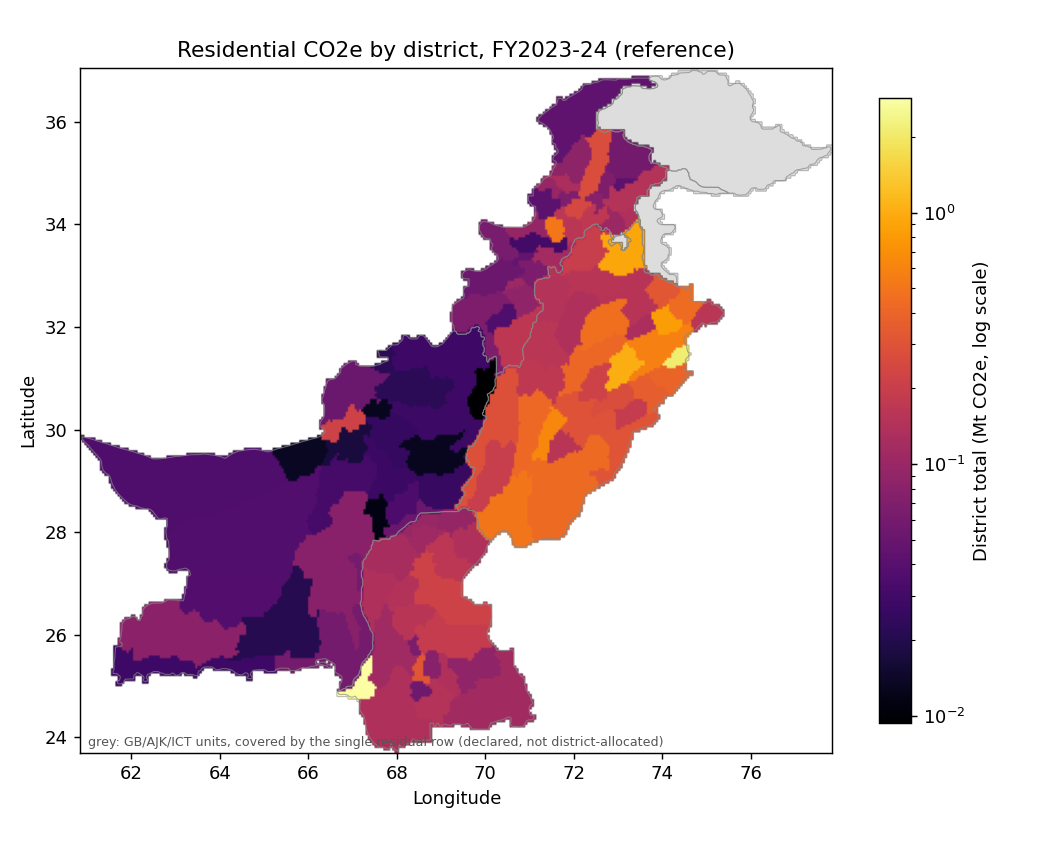
\includegraphics[width=\linewidth]{residential_district_map.png}
\caption{District allocation of residential \COe{} (reference). Each district is
painted with its allocated total; the survey's urban/rural rates on census populations
do the within-province work. The map now resolves every name through the canonical
ADM2 crosswalk: \num{114} of the \num{126} boundary polygons are painted (a polygon
carrying several census units---Karachi's seven, the Chitral and Kohistan splits---paints
their sum), and the \num{12} grey polygons are the GB/AJK/ICT units covered by the
single residual row, a declared class rather than a matching failure; every polygon's
disposition is a row of
\texttt{outputs/residential\_district\_map\_audit\_2024.csv}.
The map is presentation; the CSV is the product.}
\label{fig:districtmap}
\end{figure}

\begin{figure}[htbp]
\centering
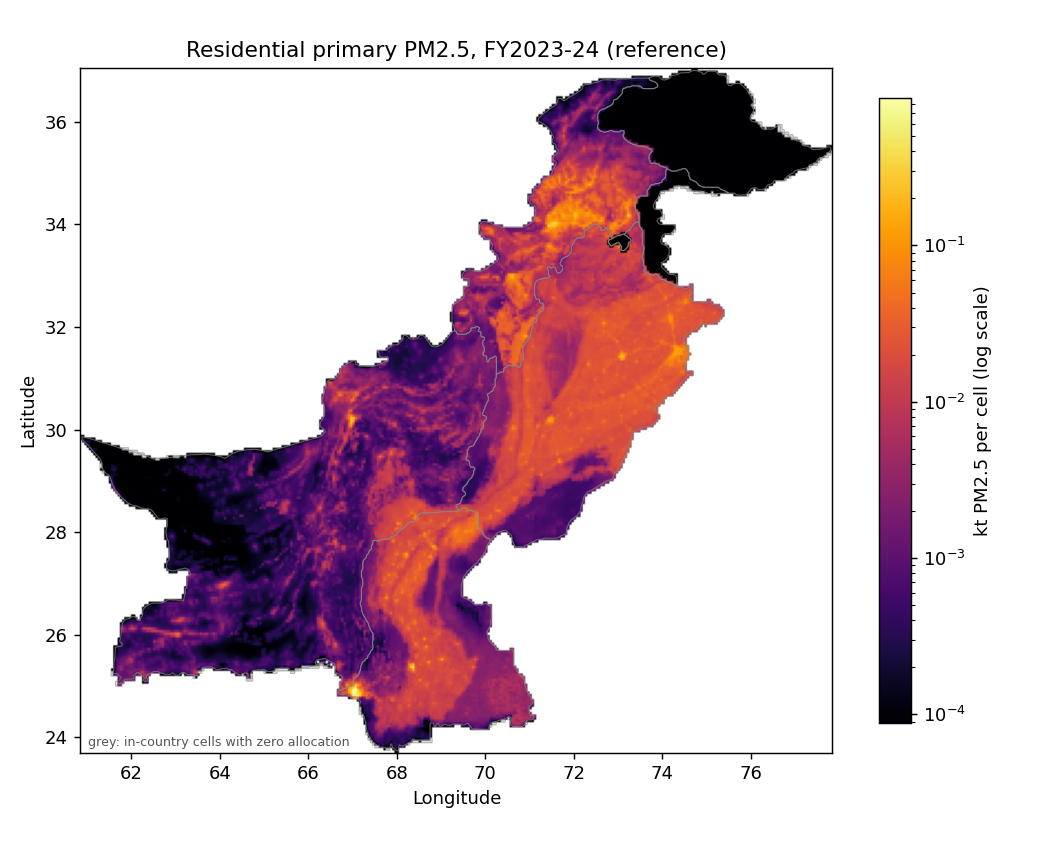
\includegraphics[width=\linewidth]{residential_map_pm25.png}
\caption{Gridded residential primary \PM{} at \SI{0.05}{\degree} (reference):
gas and generators on built-up fraction (ESA WorldCover v200~2021 class~50, CC~BY~4.0,
aggregated from \SI{10}{\metre}---a 2021 surface against FY2023--24 activity, a
declared vintage offset, hashed and documented in
\texttt{data/gis/PROXY\_SOURCES.md}), dung on livestock density, residues on
cropland, the rest on population---declared judgement, exactly reconciled to every
province and stream total. Colour is logarithmic; light grey marks in-country cells with
zero allocation (no proxy weight in that cell), distinct from the white outside the
country boundary.}
\label{fig:gridmap}
\end{figure}

\subsection{Contribution to the national inventory}

Residential fuel combustion is \SI{5.45}{\percent} of Pakistan's national emissions and
\SI{1.27}{\percent} of national Approach-1 variance---a sector whose variance share is
below its level share.

It is also almost unaffected by the cross-sector correlated-factor scenario---which,
since the common-random-numbers rebuild, moves no sector's band, transport's included:
$\pm\SI{30.4}{\percent}$ with parameters shared within the module against
$\pm\SI{30.3}{\percent}$ with factors correlated across sectors in the national Monte
Carlo (the sampled counterparts of the analytic $\pm\SI{23.1}{\percent}$ grouped figure
above). The reason is structural and worth stating as an internal check. That scenario
correlates the shared IPCC fuel-carbon factors across sectors, and this sector's uncertainty is
dominated by biomass \CHfour{} and \NtwoO{} factors that no other sector shares. A sector that
moved materially under it would indicate a factor being shared where it should not be.

\FloatBarrier
\section{Residential air-pollutant results}
\label{sec:air}
The survey-based S reference produces \SI{\SectorRefPMfine}{\kilo\tonne} primary PM$_{2.5}$ and \SI{\SectorRefBC}{\kilo\tonne} BC in FY2023--24. The latest common-core year is FY2024--25. Air mass and GHG results use the same household fuel configurations, while species-specific factors retain their own units and process definitions.

\begin{table}[htbp]\centering\small
% Native Gg; missing species are NE, not zero.
\begin{tabular}{@{}lrr@{}}\toprule
Species (Gg) & FY2023--24 & FY2024--25\\\midrule
PM$_{2.5}$ & 282.8 & 276.4 \\
BC & 20 & 19.55 \\
NO$_x$ & 156.1 & 154.2 \\
SO$_2$ & 20.84 & 20.8 \\
CO & 3354 & 3265 \\
NMVOC & 357.7 & 357.9 \\
NH$_3$ & 42.38 & 41.21 \\
\bottomrule\end{tabular}

\caption{Gross appliance emissions under reference S. BC and OC are components of PM$_{2.5}$; PM$_{10}$/TSP have narrower coal-only support.}\label{tab:air}
\end{table}

\subsection{Factors and material boundary}
Andreae biomass factors use dry fuel including ash. Dung uses total dry solids rather than ash-free volatile solids, wood is converted from survey air-dry quantity, and household residue burning is separate from field burning. Fossil gas, LPG, kerosene and coal use applicable EMEP small-combustion factors on energy. LPG's gaseous-appliance proxy and ambiguous filterable/condensable definitions remain explicit. Household generators and unusable charcoal sulfur factors remain missing estimates.

NO$_x$ is NO$_2$-equivalent throughout. Original NO factors receive the 46/30 conversion once. Pollutants are native masses and do not enter a CO$_2$-equivalent aggregate. Nested particulate species are not summed.

\subsection{Configurations and uncertainty}
S uses household dung reported by the HIES reconstruction. L assumes that all agricultural-ledger diverted dung is burned in households; the transfer establishes available material, not its destination. The alternative changes dung emissions consistently in GHG and air products, without assigning a probability to that fate. In the national FY2023--24 air panel, this case changes covered PM$_{2.5}$ from about 423 to 772 Gg.

The conditional ensemble shares household activity across pollutants. Ledger-L dung uses the same sampled herd as manure accounting, with diversion and volatile-solid assumptions held. Stove/fuel factor transfer and structural fate cases are separate from parameter intervals. The former road-factor technology endpoints are sensitivities, not a probabilistic basis for a residential/road ratio interval.

\subsection{Fitness for use}
Residential biomass is the largest covered PM$_{2.5}$ source under S, but pollutant and GHG rankings differ by specific process; there is no general inverse ordering. The source comparison is gross emitted mass, not exposure or a health-intervention ranking.

The product reports emissions at the appliance. Indoor deposition and outdoor escape are not estimated, so this mass is not an ambient-ready outdoor release. Stove location, ventilation and personal time--activity patterns would require separate evidence. Survey national/provincial controls and fixed geographic proxies support allocations rather than observed changes in local combustion. Monthly source evidence and held spatial patterns are labelled accordingly.

\FloatBarrier
% ===========================================================================
\section{Discussion}
\label{sec:discussion}
% ===========================================================================

\subsection{One sector, two emission accounts}

The central result is that this sector is \SIrange{5.4}{6.5}{\percent} of Pakistan's
greenhouse gases across the two dung configurations while carrying a configuration-
dependent but consistently leading share of its primary particulate, and that both
readings of the sector are correct.

It is tempting to resolve that tension by arguing that one accounting is wrong---that biomass
\COtwo{} should count, or that particulate should be given a \COe{} equivalent. Neither move is
defensible. The biomass memo convention is an accounting rule that prevents double
counting: biogenic \COtwo{} is held outside Energy because any net change in biomass carbon
stocks is accounted in AFOLU---whether Pakistan's fuelwood harvest is in fact balanced by
regrowth is a land-sector question this paper does not evaluate. Black carbon's metrics genuinely are contested, and converting it
would imply a comparability with long-lived gases that the science does not support.

The tension is not an artefact to be resolved but a fact about the sector: it burns a lot
of carbon whose net atmospheric effect is booked to the land sector, and emits a lot of
primary particulate. An inventory that reports only one of those describes half of it.

\subsection{What the closure buys, and what it does not}

The dung-cake transfer removes a specific failure. Before it, \SI{1.259}{\mega\tonne} of
excreted nitrogen a year left agriculture's manure balance correctly and entered nothing---an
orphaned flow that both sectors' totals were individually consistent with and that was wrong
between them.

What it does not buy is accuracy in the dung quantity itself---or even certainty that
households are the destination. The transfer guarantees that the diverted mass is
accounted for exactly once, as household combustion or as a typed unresolved remainder;
it does not establish that the \SI{28}{\percent} and
\SI{30}{\percent} burned-fuel shares are right, nor that everything they divert is burned
in dwellings. The HIES demand-side reading, a factor of \num{5.4} lower, is why the
reference books only what households report burning, why this paper
reports the all-diverted configuration beside it
(Table~\ref{tab:configs}), and why it restates the identity as
$D_{\text{diverted}} = D_{\text{residential}} + D_{\text{other/unresolved}}$. The closure
makes the two sectors share one assumption about what was diverted instead of holding two
inconsistent ones---an
improvement in consistency, while the unresolved remainder carries the open evidence
honestly.

That distinction generalises to the other closures in this inventory
\citep{ahmad2026national}: each removes an inconsistency and none removes an unknown.

\subsection{The firewood decision}

The firewood question used to be whether to include a figure carrying its source's own
estimate flag. It is now a different and better question: how far to trust a national
household survey.

The answer this sector gives is: as the primary quantity, at \SI{35}{\percent}. The HIES
total is a design-weighted measurement reproduced within \SI{6}{\percent} by an independent
round six years earlier, and the supply-side estimate it replaces lands within
\SI{7}{\percent} of it---three numbers with different biases agreeing at the ten-percent
level, which is more corroboration than most activity data in this inventory can claim. The
residual \SI{35}{\percent} prices the systematic risks a consumption survey cannot see:
recall over a one-month window, out-of-dwelling use, enterprise wood booked to households.

The honest reading of the reported figure is a range with two axes, and the
configuration axis is the wider one: \SI{24.2}{} (the reference) to
\SI{29.5}{\mega\tonne} (configuration~L), not a band
around the reference alone. Within the reference, the firewood axis spans \SI{20.8}{} to
\SI{25.4}{}, with the lower bound being the no-firewood case---which is not ``the
metered fuels alone'': it still carries the non-market dung stream, and the metered
fossil fuels by themselves support about \SI{18.4}{\mega\tonne}.

\subsection{Implications}

\textbf{Household solid fuel is the largest covered source of primary particulate.} Under
the reference and configuration L, residential combustion emits
\numrange{49}{109} times the primary \PM{} attributed to road exhaust. Ranking interventions
requires exposure, cost and abatement-effectiveness evidence that this inventory does not
provide.

\textbf{The two national surveys this sector needed both exist, and both are now held.}
HIES quantities replaced the FAOSTAT firewood estimate and supply the reference dung
quantity---a factor of five below what the nitrogen ledger diverts, with the difference
carried as unresolved rather than reconciled away. And the Multi-Tier Framework stove typology
\citep{worldbank2024mtf} supplies the national stove distribution: \SI{44.3}{\percent} of households cook mainly on clean-fuel
stoves, \SI{71.8}{\percent} of rural households on traditional or three-stone/open-fire
stoves, with stacking at \SI{6.2}{\percent}. The stove-mix sensitivity now prices that
evidence; the remaining need is the fuel-by-device-by-end-use crosswalk the report does
not publish, which is what separates this inventory from technology resolution.

\textbf{Fuel switching moves the two inventories in opposite proportions.} Replacing biomass
with piped gas would \emph{increase} this sector's reported greenhouse gases, because gas
\COtwo{} is reportable and biomass \COtwo{} is not, while sharply reducing its particulate. Any
policy evaluation that scores such a switch on the national inventory alone will score it as a
loss. That is a genuine accounting artefact rather than a physical result, and it is the
clearest case in this inventory for reporting both layers together.

% ===========================================================================
\section{Limitations}
\label{sec:limitations}
% ===========================================================================

\textbf{Firewood is a self-reported quantity, not a metered one.} The HIES total is a real
measurement---design-weighted, reproduced by an independent round, corroborated by the
supply-side estimate it replaced---but it is households reporting their own consumption over
a one-month recall, and the \SI{35}{\percent} it carries prices what such an instrument
cannot see: recall bias, out-of-dwelling use, enterprise wood booked to households. The
sector is still reported with firewood excluded and at $\pm\SI{35}{\percent}$ quantity, and
no sensitivity substitutes for a metered series that does not exist.

\textbf{The dung quantity rests on two survey rounds that disagree.} The reference takes
household dung from HIES, a per-household quantity interpolated between the 2018--19 and
2024--25 rounds: \SI{10.93}{\mega\tonne} for FY2023--24. The two rounds disagree by a
factor of \num{1.53} per household, and in 2024--25 the top 5\% of reporting households
hold \SI{44.7}{\percent} of the reported dung; the stream carries \SI{35}{\percent} for
that. The \SI{47.8}{\mega\tonne} of diverted cake the survey does not find in households
is unresolved: it sits outside the total with no emission applied, and its candidate
destinations are priced beside the total, not inside it. The diverted quantity itself
equals what agriculture's nitrogen
balance releases, exactly and by construction. That makes the two sectors consistent about
what was diverted; it does
not establish that the \SI{28}{\percent} and \SI{30}{\percent} burned-fuel shares are right,
and those come from a manure-management configuration that agriculture reports as its own
largest uncertainty.

\textbf{Supply statistics miss non-market fuels.} The fossil streams are metered and billed;
dung and firewood largely do not pass through a market and are therefore estimated rather than
counted. Firewood is the sector's largest energy stream, and the non-market biomass fuels
together supply about two-thirds of its energy.

\textbf{Biomass emission factors span more than a factor of two.} The dung and firewood methane
and nitrous oxide factors carry uncertainties above \SI{150}{\percent}, because cookstove
combustion completeness depends on stove design, fuel moisture, feeding rate and operator
behaviour, and measurement campaigns disagree. No Pakistani cookstove measurement campaign
informs these values.

\textbf{The fossil air rows are Tier~1 fleet averages with a declared PM ambiguity.} Gas,
LPG and kerosene pollutants are now estimated on the EMEP/EEA small-combustion chapter's
Tier~1 factors (the chapter is held in the repository);
the chapter's own review note---that it is unclear whether its PM factors are
filterable-only or include condensables---is quoted on the factor rows, and kerosene's
European heating-oil \SOtwo{} factor is flagged at $\pm$\SI{100}{\percent} pending a
sulfur-content route.

\textbf{The layer reports mass, not exposure.} Household combustion's health burden depends on
proximity, ventilation and time-activity patterns that a national mass inventory cannot
capture. The comparison against transport is a source ranking of gross emitted mass, not an
exposure ranking; the direction of the exposure difference is plausible but not quantified
here (Section~\ref{sec:air}).

\textbf{Short-lived forcers are reported and not counted.} Black carbon and organic
carbon are outside the \COe{} total, deliberately, because their metrics are contested;
their forcing effects oppose each other and no net effect is quantified here. The
conventional total describes only part of the sector's climate relevance.

\textbf{Firewood's within-province district and grid proxy is population.} The provincial
and urban/rural controls come from the survey's own quantities, but below them the
within-region split rides census population and the grid rides WorldPop---and firewood
availability follows forest and rangeland rather than people, so the within-province
pattern is the weakest link in its spatial chain. The national and provincial totals are
unaffected.

\textbf{The built-form bracket has three members and a named absence.} Piped gas is
allocated on the built-up fraction; the published bracket now prices that choice against
\num{2} admissible rivals---population alone, and the renormalised product of built-up and
population---and all three are structurally invariant at district level because the
district panel fixes each shape's mass. The choice matters only at the grid cell, where
the bracket's spread is published as a per-cell magnitude rather than a district price.
The fourth member the ensemble wants---a surface separating residential from
non-residential built area---is not held: it is recorded as a named acquisition
(EMC-BUILT) rather than approximated by what is on hand.

\textbf{Mixed vintages inside one sector.} The fossil streams are FY2023--24 while
firewood rides the 2024--25 survey round and the dung-cake stream a per-household rate
interpolated between the two rounds. Stated rather than smoothed over.

\textbf{Historical support differs by fuel.} The common core covers FY2015--16 through FY2024--25. Gas uses observed annual OGRA deliveries; survey dung and firewood interpolate or extrapolate household quantities between HIES rounds, and residues follow crop production. Carried LPG, kerosene and minor-stream quantities remain labelled, rather than being called annual observations. Before the first survey anchor, a held per-household rate is an assumption rather than a measured trend.

% ===========================================================================
\section{Conclusion}
\label{sec:conclusion}
% ===========================================================================

Pakistani households emitted \SIrange{24.2}{29.5}{\mega\tonne} \COe{} in FY2023--24
across the survey-based reference and the all-diverted dung configuration---where the
diverted dung that households do not report burning goes is the sector's dominant open
question---plus biogenic \COtwo{} reported
outside the total. The same combustion emitted \SIrange{283}{632}{\kilo\tonne} of gross
primary \PM{}: under either configuration the sector is among the country's largest
primary-particulate sources, at \numrange{49}{109} times road transport's
exhaust particulate, from a sector less than half road transport's size in \COe{}.

Three results generalise. First, one sector can be minor in a climate inventory and
dominant in a primary-emission inventory, and both readings can be right: the biomass
memo convention holds biogenic \COtwo{} outside national totals while counting the
methane and nitrous oxide of incomplete combustion, so a country selecting air-quality
interventions from a greenhouse-gas ranking will systematically under-prioritise the
sources that matter most for health. Second, computing both emission layers from one
activity basis is what makes their comparison meaningful: under matched years and the
stated definitions, the particulate ratio reflects combustion and fuel quantities
rather than which datasets two authors happened to hold. Third, a cross-sector
transfer should be a derivation rather than a second estimate---and a conservation
constraint should never be mistaken for destination evidence: the ledger fixes what
agriculture diverted, the survey observes what households burned, and the
factor-of-five gap between them is reported as the open question it is.

Both national surveys this sector needed turned out to exist. HIES replaced the
flagged FAOSTAT firewood figure with a twice-corroborated measurement and exposed the
dung disagreement; the Multi-Tier Framework stove typology \citep{worldbank2024mtf}
feeds the technology-mix sensitivity. What remains for full resolution is the
fuel-by-device-by-end-use crosswalk, Pakistani emission measurements, and the exposure
layer this paper's scope deliberately excludes.

\FloatBarrier

% ---------------------------------------------------------------------------
\section*{Code and data availability}
% ---------------------------------------------------------------------------

The calculation engine, the activity data and every output quoted here are version-controlled
in the inventory repository (\url{https://github.com/RehanAhmad13/pakistan-emissions-sectors})
and reproduce from a single command. The sector is regenerated with
\texttt{python3 -m pkinv.sectors.residential.run\_residential}; \ref{app:repro} gives the full
sequence. Every number printed in this paper is read from a generated CSV rather than
transcribed, and a test asserts that the manuscript and the engine agree.

% ---------------------------------------------------------------------------
\bibliographystyle{elsarticle-harv}
\bibliography{../../paper_common/references}

% ---------------------------------------------------------------------------
\appendix
\renewcommand{\thetable}{\arabic{table}}%
\renewcommand{\thefigure}{\arabic{figure}}%
% Each appendix is barriered: these are wide table* floats, which cannot be placed
% on the page that introduces them, so without a barrier they queue behind one
% another and flush across near-blank pages away from their own headings.
% ===========================================================================
\section{Reproduction}
\label{app:repro}
% ===========================================================================

The sector runs on Python 3.11 with no compiled dependencies. From the repository
root:

{\footnotesize
\begin{verbatim}
pip install -e .
python3 -m pkinv.sectors.residential.run_residential
python3 -m unittest discover tests
\end{verbatim}
}

The first command runs every layer of the sector in sequence---the greenhouse-gas
engine, the air-pollutant layer, the survey comparison, the official benchmarks and
CCAC bridge, the uncertainty module, the district allocation, the time series and
the monthly profiles---and prints the dung-cake nitrogen closure as it runs. Its outputs land
in \texttt{outputs/}, and this is which is which---the list they replace named them
collectively as \texttt{residential\_*.csv}, which told a reader what exists without giving a
filename for any of it:

\begin{itemize}\itemsep2pt
\item \texttt{residential\_\allowbreak totals\_\allowbreak 2024.csv}: the sector total under the reference, with configuration L beside it and the sector's mixed input vintages stated on the row rather than smoothed over.
\item \texttt{residential\_\allowbreak by\_\allowbreak stream\_\allowbreak 2024.csv}: the same total by fuel stream.
\item \texttt{residential\_\allowbreak fuel\_\allowbreak 2024.csv}: the energy behind those streams in TJ and share.
\item \texttt{residential\_\allowbreak provincial\_\allowbreak 2024.csv}: the provincial split, and \texttt{residential\_\allowbreak district\_\allowbreak 2024.csv} the district allocation beneath it.
\item \texttt{residential\_\allowbreak strata\_\allowbreak 2024.csv}: the allocation basis: fuel by province and rural or urban stratum, on the survey's own strata.
\item \texttt{residential\_\allowbreak monthly\_\allowbreak 2024.csv}: the monthly profile, and \texttt{residential\_\allowbreak emissions\_\allowbreak monthly\_\allowbreak 2024.csv} the emissions it carries.
\item \texttt{residential\_\allowbreak air\_\allowbreak pollutants\_\allowbreak 2024.csv}: the air-pollutant layer, and \texttt{residential\_\allowbreak pm\_\allowbreak ratio\_\allowbreak 2024.csv} the residential-over-road primary \PM{} ratio with its parametric interval.
\item \texttt{residential\_\allowbreak hies\_\allowbreak comparison\_\allowbreak 2024.csv}: the survey comparison, this inventory's quantities against the HIES round that anchors them.
\item \texttt{residential\_\allowbreak official\_\allowbreak comparison\_\allowbreak 2024.csv}: the official benchmarks, and \texttt{residential\_\allowbreak unfccc\_\allowbreak crt\_\allowbreak cell\_\allowbreak audit\_\allowbreak 2024.csv} the CRT cell extraction behind them.
\item \texttt{residential\_\allowbreak ccac\_\allowbreak bridge\_\allowbreak 2024.csv}: the CCAC bridge, item by item in \PM{} terms.
\item \texttt{residential\_\allowbreak uncertainty\_\allowbreak 2024.csv}: the interval; \texttt{residential\_\allowbreak uncertainty\_\allowbreak inputs\_\allowbreak 2024.csv} the input register behind it; \texttt{residential\_\allowbreak uncertainty\_\allowbreak scenarios\_\allowbreak 2024.csv} the structural scenarios.
\item \texttt{residential\_\allowbreak dung\_\allowbreak ledger\_\allowbreak 2024.csv}: the dung-cake closure the run prints: each claimant's air-dry mass, its share of the diverted quantity and how it is treated.
\item \texttt{residential\_\allowbreak timeseries.csv}: the series across years.
\item \texttt{residential\_\allowbreak qa\_\allowbreak 2024.csv}: the quality-control report.
\end{itemize}

Figures regenerate with \texttt{pkinv.report.figures} and are copied into this manuscript by
\texttt{scripts/sync\_figures.py}.

The dung stream's diverted quantity is derived from the agriculture sector's nitrogen
flow, so reproducing it requires that sector's data to be loadable; the equality of the
two sectors' nitrogen is asserted by \texttt{tests/test\_residential.py} with
\texttt{==} rather than a tolerance, and the destination configurations (L/S) share
that quantity.

The HIES microdata are not redistributed here: the SPSS files are fetched from the
Pakistan Bureau of Statistics microdata portal and hash-pinned in a manifest, and
only the derived, design-weighted aggregate tables are committed. Every other
input is committed directly, and a run manifest hashes the held sources.

% ===========================================================================
\section{Sources}
\label{app:sources}
% ===========================================================================

Natural gas and LPG supplied to households are OGRA's sector-wise tables
\citep{ogra2024}, with the nine-edition archive \citep{ograarchive} behind the
time series; household kerosene is OCAC's sectoral sales \citep{ocacaviation}.
Firewood is the HIES 2024--25 design-weighted household quantity \citep{hies2025},
with the 2018--19 round \citep{hies2019} as an independent check and FAOSTAT's
wood-fuel series \citep{faostat} retained only as a structural scenario, carrying
FAO's own estimate flag. Household dung cake is the HIES quantity, a per-household
rate interpolated between the two rounds \citep{hies2019,hies2025}; the diverted
quantity it is set against, and configuration L, are derived from the agriculture sector's
nitrogen balance rather than from any external source, with cake ash and moisture
from proximate-analysis literature \citep{szymajda2019}. Greenhouse-gas factors
are IPCC 2006 Guidelines Volume~2 Chapter~2 Table~2.5 \citep{ipcc2006stationary};
air-pollutant factors are the Andreae compilation \citep{andreae2019}, the
EMEP/EEA small-combustion chapter \citep{emep2023smallcombustion}, the Akagi
compilation \citep{akagi2011}, and the field-burning mirrors \citep{emep2019} for
crop residues. Degree-days derive from NASA POWER monthly temperature
\citep{nasapower}; the generator stream uses the Government of Pakistan's
administered petrol prices \citep{goppetrol}. External comparisons are EDGAR
\citep{edgar2025booklet}, Pakistan's CRT workbook \citep{pakcrt2026}, BUR-1
\citep{pakbur1} and the CCAC/SEI assessment \citep{ccacsei2023}.

\FloatBarrier
% ===========================================================================
\section{Supplementary Note: the dung-cake closure}
\label{app:dung}
% ===========================================================================

The design decision worth recording is what the ledger conserves and what it leaves
open. It conserves the DIVERTED quantity: agriculture removes \SI{28}{\percent} of
cattle and \SI{30}{\percent} of buffalo excreted nitrogen from its manure-management
balance and books it IE to Energy, and this sector receives exactly that quantity---not
an independent estimate that would then need ongoing reconciliation, whose failure mode
is silent (both sectors' totals stay internally consistent while the flow between them
does not balance). What the ledger does NOT settle is the destination of the diverted
mass. The household survey observes \SI{11.97}{\mega\tonne} of cake consumed in
dwellings in its 2024--25 round, a factor of \num{4.9} below the diverted total, and the
series interpolated between its two rounds puts \SI{10.93}{} there in FY2023--24. The
paper reads the
destination two ways: the reference books the observed household
consumption and carries the remainder as
$D_{\text{other/unresolved}}$, outside the total with no emission applied, and
configuration L, the reference of earlier releases, books it all to
household combustion (Section~\ref{sec:results}).

The diverted quantity itself is derived from agriculture's nitrogen flow:
\begin{equation}
M_{\mathrm{VS}} \;=\; \sum_{a} N_a \, f_a \, \frac{\mathrm{VS}_a}{\mathrm{Nex}_a},
\end{equation}
using the same herd, the same species categories, the same burned-fuel shares $f_a$, and
IPCC's volatile-solids and nitrogen-excretion rates for the same animal categories and region.
The result is \SI{1.259}{\mega\tonne} of nitrogen corresponding to
\SI{38.77}{\mega\tonne} of ash-free volatile solids---the ledger intermediate, not a
burnable fuel mass---and a test asserts the correspondence with \texttt{==} rather than
a tolerance.

Three masses follow from that one intermediate, and each pairs with its own factor basis:
total dry solids restore the mineral ash a hand-formed cake carries
($\mathrm{TS} = \mathrm{VS}/(1-\text{ash})$, \SI{51.69}{\mega\tonne}) and are the basis
Andreae's per-kilogram-dry-fuel pollutant factors describe; air-dry cake mass restores the
equilibrium moisture ($\mathrm{TS}/(1-\text{moisture})$, \SI{58.74}{\mega\tonne}) and
pairs with IPCC's as-received net calorific value for the energy calculation. These are
the masses of the diverted supply, and of the stream configuration L burns; the reference
reads air-dry cake from the survey and removes the same moisture fraction for its dry
mass (Table~\ref{tab:massbases}). The
superseded pairing---ash-free volatile solids on the as-received NCV, a three-bases
conflation that understated the stream---is retained only as the structural scenario
\texttt{dung\_basis\_legacy\_vs}.

The property this buys is not accuracy but the impossibility of a particular error. If
agriculture's manure-management shares change, the diverted quantity changes with them,
in the same commit, and neither sector can be updated into inconsistency with the other
about what was diverted. Where the part of that quantity households do not report
burning goes
remains the sector's dominant open question, carried explicitly rather than resolved by
construction.

\FloatBarrier
% GENERATED by scripts/make_residential_factor_table.py - do not hand-edit;
% tests/test_residential_crt.py asserts this file matches the factor data.
% ===========================================================================
\section{Supplementary Table: every air-pollutant factor the layer burns}
\label{app:factors}
% ===========================================================================

Basis rules, stated once: biomass factors are per kilogram of dry fuel
including ash (total dry solids for dung, oven-dry for firewood, dry matter
for residues, as-purchased for charcoal); fossil factors are per gigajoule of
fuel energy; black carbon is reported INSIDE PM$_{2.5}$, never additional to
it; NO$_x$ is reported as NO$_2$-equivalent throughout---sources publishing
as~NO (the Andreae rows) are converted $\times 46/30$ on their data rows, so
one basis sums; the device is a single implicit class per fuel---the
traditional/open class that dominates rural biomass cooking (71.8\% of rural
households per the MTF 2021--22 stove typology; the fuel-by-device crosswalk
needed for full technology resolution is not yet published). All
values are gross emission at the appliance. Flags: c~=~the source's own
filterable-versus-condensable caveat is quoted on the data row; d~=~the
printed confidence interval is defective and the row carries $\pm$100 with
the bounds quoted; s~=~a sulfur-content assumption is stated on the row.

\begin{table*}[htbp]
\centering
\scriptsize
\begin{tabular}{@{}llrlllr@{}}
\toprule
\textbf{Pollutant} & \textbf{Fuel} & \textbf{Value} & \textbf{Unit} & \textbf{Source} & \textbf{Flags} & \textbf{$\pm$\%} \\
\midrule
PM$_{2.5}$ & Charcoal & 18.7 & g/kg dry & Andreae 2019 & -- & 85 \\
PM$_{2.5}$ & Coal & 398 & g/GJ & EMEP/EEA 2023 ch.\,1.A.4 & c & 51 \\
PM$_{2.5}$ & Crop residues & 7.6 & g/kg dry & Andreae 2019 & -- & 50 \\
PM$_{2.5}$ & Dung cake & 8.3 & g/kg dry & Andreae 2019 & -- & 40 \\
PM$_{2.5}$ & Firewood & 6.7 & g/kg dry & Andreae 2019 & -- & 49 \\
PM$_{2.5}$ & Kerosene & 1.9 & g/GJ & EMEP/EEA 2023 ch.\,1.A.4 & c & 39 \\
PM$_{2.5}$ & LPG & 1.2 & g/GJ & EMEP/EEA 2023 ch.\,1.A.4 & c & 42 \\
PM$_{2.5}$ & Natural gas & 1.2 & g/GJ & EMEP/EEA 2023 ch.\,1.A.4 & c & 42 \\
PM$_{10}$ & Coal & 404 & g/GJ & EMEP/EEA 2023 ch.\,1.A.4 & c & 50 \\
TSP & Coal & 444 & g/GJ & EMEP/EEA 2023 ch.\,1.A.4 & c & 59 \\
BC & Charcoal & 0.43 & g/kg dry & Andreae 2019 & -- & 49 \\
BC & Crop residues & 0.5 & g/kg dry & Akagi 2011 & -- & 60 \\
BC & Dung cake & 0.51 & g/kg dry & Andreae 2019 & -- & 67 \\
BC & Firewood & 0.53 & g/kg dry & Andreae 2019 & -- & 66 \\
BC & Gaseous fuels & 0.054 & frac.\ of PM$_{2.5}$ & EMEP/EEA 2023 ch.\,1.A.4 & -- & 77 \\
BC & Liquid fuels & 0.085 & frac.\ of PM$_{2.5}$ & EMEP/EEA 2023 ch.\,1.A.4 & -- & 72 \\
BC & Solid fuels & 0.064 & frac.\ of PM$_{2.5}$ & EMEP/EEA 2023 ch.\,1.A.4 & d & 100 \\
OC & Charcoal & 5.9 & g/kg dry & Andreae 2019 & -- & 42 \\
OC & Crop residues & 3.3 & g/kg dry & Akagi 2011 & -- & 60 \\
OC & Dung cake & 4.4 & g/kg dry & Andreae 2019 & -- & 43 \\
OC & Firewood & 3.0 & g/kg dry & Andreae 2019 & -- & 50 \\
CO & Charcoal & 207 & g/kg dry & Andreae 2019 & -- & 30 \\
CO & Coal & 4600 & g/GJ & EMEP/EEA 2023 ch.\,1.A.4 & -- & 43 \\
CO & Crop residues & 92 & g/kg dry & IPCC 2006 V4 (mirror) & -- & 40 \\
CO & Dung cake & 89 & g/kg dry & Andreae 2019 & -- & 47 \\
CO & Firewood & 83 & g/kg dry & Andreae 2019 & -- & 35 \\
CO & Kerosene & 57 & g/GJ & EMEP/EEA 2023 ch.\,1.A.4 & -- & 40 \\
CO & LPG & 26 & g/GJ & EMEP/EEA 2023 ch.\,1.A.4 & -- & 46 \\
CO & Natural gas & 26 & g/GJ & EMEP/EEA 2023 ch.\,1.A.4 & -- & 46 \\
NO$_x$ & Charcoal & 1.81 & g/kg dry & Andreae 2019 & -- & 73 \\
NO$_x$ & Coal & 110 & g/GJ & EMEP/EEA 2023 ch.\,1.A.4 & -- & 75 \\
NO$_x$ & Crop residues & 2.5 & g/kg dry & IPCC 2006 V4 (mirror) & -- & 50 \\
NO$_x$ & Dung cake & 4.29 & g/kg dry & Andreae 2019 & -- & 46 \\
NO$_x$ & Firewood & 3.83 & g/kg dry & Andreae 2019 & -- & 52 \\
NO$_x$ & Kerosene & 51 & g/GJ & EMEP/EEA 2023 ch.\,1.A.4 & -- & 40 \\
NO$_x$ & LPG & 51 & g/GJ & EMEP/EEA 2023 ch.\,1.A.4 & -- & 39 \\
NO$_x$ & Natural gas & 51 & g/GJ & EMEP/EEA 2023 ch.\,1.A.4 & -- & 39 \\
NMVOC & Charcoal & 6.6 & g/kg dry & Andreae 2019 & -- & 74 \\
NMVOC & Coal & 484 & g/GJ & EMEP/EEA 2023 ch.\,1.A.4 & -- & 61 \\
NMVOC & Crop residues & 7.0 & g/kg dry & Akagi 2011 & -- & 60 \\
NMVOC & Dung cake & 14.4 & g/kg dry & Andreae 2019 & -- & 70 \\
NMVOC & Firewood & 7.8 & g/kg dry & Andreae 2019 & -- & 64 \\
NMVOC & Kerosene & 0.69 & g/GJ & EMEP/EEA 2023 ch.\,1.A.4 & -- & 43 \\
NMVOC & LPG & 1.9 & g/GJ & EMEP/EEA 2023 ch.\,1.A.4 & -- & 39 \\
NMVOC & Natural gas & 1.9 & g/GJ & EMEP/EEA 2023 ch.\,1.A.4 & -- & 39 \\
SO$_2$ & Coal & 900 & g/GJ & EMEP/EEA 2023 ch.\,1.A.4 & s & 39 \\
SO$_2$ & Crop residues & 0.40 & g/kg dry & EMEP/EEA 2019 (mirror) & -- & 70 \\
SO$_2$ & Dung cake & 0.77 & g/kg dry & Andreae 2019 & -- & 48 \\
SO$_2$ & Firewood & 0.47 & g/kg dry & Andreae 2019 & -- & 94 \\
SO$_2$ & Kerosene & 70 & g/GJ & EMEP/EEA 2023 ch.\,1.A.4 & d,s & 100 \\
SO$_2$ & LPG & 0.3 & g/GJ & EMEP/EEA 2023 ch.\,1.A.4 & -- & 33 \\
SO$_2$ & Natural gas & 0.3 & g/GJ & EMEP/EEA 2023 ch.\,1.A.4 & -- & 33 \\
NH$_3$ & Charcoal & 2.5 & g/kg dry & Andreae 2019 & -- & 70 \\
NH$_3$ & Coal & 0.3 & g/GJ & EMEP/EEA 2023 ch.\,1.A.4 & d & 100 \\
NH$_3$ & Crop residues & 1.3 & g/kg dry & Akagi 2011 & -- & 60 \\
NH$_3$ & Dung cake & 1.33 & g/kg dry & Andreae 2019 & -- & 59 \\
NH$_3$ & Firewood & 0.89 & g/kg dry & Andreae 2019 & -- & 55 \\
\bottomrule
\end{tabular}
\caption{The complete air-pollutant factor set, generated from the factor
file the engine reads (\texttt{data/emission\_factors.csv}). Omissions are
deliberate and declared in the text: charcoal SO$_2$ (unusable source cell),
NH$_3$ for gaseous and liquid fuels (not applicable in the chapter's tables),
and every generator pollutant (no household-genset factor class exists).}
\label{tab:factors}
\end{table*}

\FloatBarrier
% GENERATED by scripts/make_residential_completeness_table.py - do not
% hand-edit; a test asserts this file matches the engine's completeness table.
% ===========================================================================
\section{Supplementary Table: the 1.A.4.b completeness matrix}
\label{app:completeness}
% ===========================================================================

Every category--gas combination the sector might contain, with its IPCC
notation key and the justification the engine carries for every non-E entry.
Generated from the same completeness table the national inventory publishes,
which is itself synced to the gap register by test.

\begin{table*}[htbp]
\centering
\scriptsize
\begin{tabular}{@{}lclp{0.52\linewidth}@{}}
\toprule
\textbf{Category} & \textbf{Key} & \textbf{Gases} & \textbf{Justification (abridged)} \\
\midrule
piped natural gas & E & CO2/CH4/N2O & OGRA sector-wise gas consumption (FY2023-24, 821 MMCFD) x IPCC Vol 2 Ch 2 Table 2.5, the Residential table - not the Energy Industries table used by 1.A.1.a. \\[2pt]
LPG & E & CO2/CH4/N2O & OGRA national supply x a domestic share read from OGRA Figure 5.2, which is published only as a bar chart. \\[2pt]
kerosene & E & CO2/CH4/N2O & OCAC total SKO, treated in full as household use; an upper bound, but under 0.2 Mt CO2e either way. \\[2pt]
dung cake & E & CH4/N2O & The household survey's quantity (HIES 2018-19 and 2024-25, per-household rate interpolated). The IE transfer above is the diverted supply it is set against; the part with no household destination is unresolved and outside the total. Biogen\ldots \\[2pt]
firewood & E & CH4/N2O & HIES 2024-25 design-weighted household quantity: 23.1 Mt air-dry wood, a measurement replacing FAOSTAT's flagged, unmoving estimate. Twice corroborated - HIES 2018-19 agrees within 6\%, FAOSTAT's moisture-matched equivalent within 7\% - an\ldots \\[2pt]
biogenic CO2 (dung cake, firewood, residues, charcoal) & IE & CO2 & Memo item, outside the national total, per IPCC's biomass convention and Pakistan's own BUR-1. Any net stock loss belongs in LULUCF. \\[2pt]
electricity & IE & - & Household electricity is nearly half of national consumption and is counted at the point of generation in 1.A.1.a. Deliberately absent; a test asserts no electricity stream exists. \\[2pt]
coal and charcoal & E & CO2/CH4/N2O & HIES 2024-25 design-weighted quantities - 13.2 kt coal, 8.3 kt charcoal, each on about one household in a thousand, three orders below firewood. OGRA's nil household coal row was roughly right for the wrong reason (a quantity too small for\ldots \\[2pt]
crop residues and cotton sticks & E & CH4/N2O & An upper-bound residential allocation of the agriculture residue ledger's fuel destination: frac\_fuel covers all fuel use (R\_fuel = R\_household + R\_commercial/industrial + R\_unresolved), and the whole 9.3 Mt dry (10.5 Mt air-dry) is b\ldots \\[2pt]
petrol generators & E & CO2/CH4/N2O & HIES 2024-25 generator-fuel expenditure over the administered petrol price: 56 kt of petrol, 2,495 TJ, 0.17 Mt CO2e. Carved out of the road-transport petrol control through the same relayed-accessor idiom as railway diesel, asserted with e\ldots \\[2pt]
biogas digesters & NE & CH4 & Domestic biogas digesters exist in Pakistan (PCRET-supported units, cattle-belt provinces); the programme installation records that would count them have not been obtained here, and HIES carries no biogas consumption item to fall back on.\ldots \\[2pt]
charcoal production wood & NE & CO2/CH4 & The 8.3 kt of charcoal burned implies roughly 35-50 kt of wood carbonised upstream (4-6 kg wood per kg charcoal), with kiln CH4 that IPCC books to the producing category. No Pakistani charcoal-production statistic exists; the quantity is b\ldots \\[2pt]
\bottomrule
\end{tabular}
\caption{The residential completeness matrix, generated from the engine
(\texttt{outputs/completeness.csv}, 1.A.4.b rows). Full justifications,
including the magnitudes that bound each NE entry where a comparator exists,
are in the generated national table.}
\label{tab:completeness144b}
\end{table*}

\FloatBarrier
% GENERATED by scripts/make_residential_air_matrix.py - do not hand-edit;
% a test regenerates this file and asserts the committed copy matches.
% ===========================================================================
\section{Supplementary Table: the air-pollutant completeness matrix}
\label{app:airmatrix}
% ===========================================================================

Every stream--pollutant combination, E derived from the air layer's actual
rows (the matrix cannot claim coverage the engine does not compute) and every
NE carrying its declared reason, keyed below the table. All estimated cells
are gross emitted mass at the appliance, on the reference (household-survey) quantity for the dung row.

\begin{table*}[htbp]
\centering
\scriptsize
\setlength{\tabcolsep}{4pt}
\begin{tabular}{@{}lcccccccccc@{}}
\toprule
\textbf{Stream} & PM$_{2.5}$ & PM$_{10}$ & TSP & BC & OC & CO & NO$_x$$^{n}$ & NMVOC & SO$_2$ & NH$_3$ \\
\midrule
Natural gas & E & NE$^{a}$ & NE$^{b}$ & E & NE$^{c}$ & E & E & E & E & NE$^{d}$ \\
LPG & E & NE$^{a}$ & NE$^{b}$ & E & NE$^{c}$ & E & E & E & E & NE$^{e}$ \\
Kerosene & E & NE$^{a}$ & NE$^{b}$ & E & NE$^{c}$ & E & E & E & E & NE$^{f}$ \\
Coal & E & E & E & E & NE$^{c}$ & E & E & E & E & E \\
Generators & NE$^{g}$ & NE$^{g}$ & NE$^{g}$ & NE$^{g}$ & NE$^{g}$ & NE$^{g}$ & NE$^{g}$ & NE$^{g}$ & NE$^{g}$ & NE$^{g}$ \\
Dung cake & E & NE$^{a}$ & NE$^{b}$ & E & E & E & E & E & E & E \\
Firewood & E & NE$^{a}$ & NE$^{b}$ & E & E & E & E & E & E & E \\
Charcoal & E & NE$^{a}$ & NE$^{b}$ & E & E & E & E & E & NE$^{h}$ & E \\
Crop residues & E & NE$^{a}$ & NE$^{b}$ & E & E & E & E & E & E & E \\
Biogas & NE$^{i}$ & NE$^{i}$ & NE$^{i}$ & NE$^{i}$ & NE$^{i}$ & NE$^{i}$ & NE$^{i}$ & NE$^{i}$ & NE$^{i}$ & NE$^{i}$ \\
\bottomrule
\end{tabular}
\caption{The air-pollutant completeness matrix. $^{n}$NO$_2$-equivalent
basis throughout. NE reasons:
$^{a}$~Andreae tabulates TPM, not PM10; the coarse fraction is not adopted for biomass and the gaseous/liquid chapters' PM10 adds nothing above PM2.5 for premixed flames.
$^{b}$~as PM10: not adopted for biomass; the coal row is the one solid fuel with a chapter TSP factor.
$^{c}$~no OC factor adopted for this stream.
$^{d}$~not applicable in the chapter's gaseous-fuel table; omitted, never zero-filled.
$^{e}$~not applicable in the chapter's gaseous-fuel table.
$^{f}$~not applicable in the chapter's liquid-fuel table.
$^{g}$~no household-genset factor class exists in the held EMEP chapter; declared omission bounded by the stream's 56 kt of fuel (the non-road small-engine chapter is the registered upgrade).
$^{h}$~the source cell prints a range its own average falls outside, on two measurements - unusable, omitted rather than guessed.
$^{i}$~the stream itself is NE (no digester count exists; see the completeness matrix and residential-biogas in the gap register).
}
\label{tab:airmatrix}
\end{table*}

\FloatBarrier

\end{document}
